% declare documents and packages
\documentclass[man, 12pt, a4paper, nolmodern, noextraspace]{apa6}
\usepackage[T1]{fontenc}
\usepackage[utf8]{inputenc}
\usepackage[american]{babel}
\usepackage{csquotes}
\usepackage{amsmath}
\usepackage{microtype}
\usepackage{caption}
\usepackage{subcaption}
\usepackage{graphicx}
\usepackage{url}
\usepackage{times}
\usepackage{booktabs}
\usepackage{multirow} % multirow tables
\usepackage{arydshln} % dashline in tabular 
\usepackage{rotating} % vertical tables
\usepackage{pdflscape} % landscape pages
\renewcommand{\footnotesize}{\small} % use 11pt for footnotes
\usepackage[doublespacing]{setspace} % single space for footnotes
%\setlength{\skip\footins}{1.5pc plus 1pt} % some more space between footnote and main body
% this command put all footnotes to endnote at the end of the paper
\usepackage{endnotes}
\let\footnote\endnote

% for word counts
\newcommand{\detailtexcount}{%
  \immediate\write18{texcount -merge -sum -incbib -dir \jobname.tex > \jobname.wcdetail }%
  \verbatiminput{\jobname.wcdetail}%
}
\newcommand{\quickwordcount}{%
  \immediate\write18{texcount -1 -sum -merge \jobname.tex > \jobname-words.sum }%
  \input{\jobname-words.sum} words%
}
\newcommand{\quickcharcount}{%
  \immediate\write18{texcount -1 -sum -merge -char \jobname.tex > \jobname-chars.sum }%
  \input{\jobname-chars.sum} characters (not including spaces)%
}

% Biblatex
\usepackage[style=apa,sortcites=true,sorting=nyt,backend=biber,uniquename=false]{biblatex}
\AtEveryBibitem{%
  \clearfield{issn} % Remove issn
  \clearfield{doi} % Remove doi
  }
% make in-text citations clickable
\usepackage[colorlinks=true]{hyperref}
% this removes annoying colors for in-text citation entries 
\usepackage{xcolor}
\hypersetup{  
    colorlinks,
    linkcolor={red!50!black},
    citecolor={blue!50!black},
    urlcolor={blue!80!black}
}

\addbibresource{abm_misinformation_lit.bib}
\DeclareLanguageMapping{american}{american-apa}
 
\title{If you see something, then say something to others: Complex contagions and the socially-contingent correction of misinformation}

\shorttitle{Socially-contingent corrections}


\author{\addvspace{.25in} Hyunjin Song}

\affiliation{Department of Communication, University of Vienna, Austria}

\abstract{As the citizens' news consumption is increasingly driven by online sources, the propagation of misinformation and so-called \enquote{fake news} on those platforms become an increasing concern for the public and policy makers. Our goal in this contribution is to offer a more systematic assessment of underlying mechanisms of misinformation spreading and its correction, combining a macro social contextual factor and individuals' cognitive basis of adopting misinformation into a more integrated, dynamic system model perspective. We first review existing evidence concerning individuals' cognitive basis of adopting such misinformation, and social context of which exposure to misinformation and its corrections are received. Next, adopting a well-known class of an epidemic model of virus infection and recovery, we combine this micro and macro dynamics into comprehensive, integrated model of misinformation diffusion on social networks. We do so by focusing on the distinction between simple contagion of misinformation vs. complex contagion of adopting corrective messages. Relying on Agent-based simulations, we further explore various boundary conditions of such dynamics, aiming to uncover how and when such misinformation propagates into the public, as well as what factors facilitate or hinder such diffusion process.}

\keywords{Misinformation, fake news, correction, simple contagion, complex contagion, exponential random graph model, agent-based simulations}


\authornote{ Hyunjin (Jin) Song is currently an assistant professor ("Universitätsassistent, post-doc") in the Department of Communication at the University of Vienna, and also a member of the Vienna Computational Communication Science Lab. Please direct any questions and inquiries concerning this manuscript to \href{mailto:hyunjin.song@univie.ac.at}{hyunjin.song@univie.ac.at}}

\note{\addvspace{.25in} 
Word count: 8908 words \\
Draft date: \today \\
\addvspace{1in} 
Paper prepared for presentation at the 2018 Annual Conference of the International Communication Association (ICA), Prague, Czech Republic, May 24 -- 28, 2018 \\
\addvspace{.25in} 
      \textbf{Draft in progress. Please do not cite without permission.} \\
      }

\begin{document}
\setcounter{page}{0}
\maketitle
  Citizens across the worlds are experiencing major changes in their news environments with the development of digital media. One of the most dramatic changes in the news environment in recent decades involves the role social networking sites (SNS) such as Facebook and Twitter play as a primary source of news outlets. Not only citizens' news consumptions are increasingly driven by such online sources \parencite{shearer2017news}, but it also appears that citizens themselves are actively participating in news dissemination on those platforms by sharing news with their peers \parencite[e.g.,][]{shearer2017news, lee2017people}. 

  An effective deliberation among public is regarded as a keystone of thriving democracies, and modern political systems squarely depend  on  informed  decisions of citizens in that regard \parencite{carpini1996}. Yet, a propagation of rumors, misinformation, and so-called \enquote{fake news} on those platforms becomes an increasing concern for the public and policy makers alike \parencite{allcott2017social, lazer2017combating}, as evidenced in recent 2016 U.S. presidential election \parencite{guess2018selective, giglietto2016fakes, allcott2017social} and in Brexit votes \parencite{nyt_2017}. While a wide circulation of factually dubious information is not entirely new to political arena, a growing trend of digitally disseminated rumors and misinformations -- often termed as a \enquote{fake news} phenomenon -- is increasingly recognized as a serious threat to liberal democratic societies \parencite{allcott2017social, lazer2017combating}. Either based on unsubstantiated rumors or based on factually wrong beliefs, many of the misinformed behave differently than those who are accurately informed \parencite{kuklinski2000misinformation}. They often disagree about basic facts about many public issues, and continue to believe and rely on such false information when making political judgments \parencite{nyhan2010corrections,thorson_2016}. 

  Along with these trends, there has been an growing interest among scholars on how people process and maintain factually false (or at least dubious) information from an individual's cognitive processing perspectives \parencite{Lewandowsky_2012PSPI, kuklinski2000misinformation, weeks2015emotions}. These studies have generated a valuable insights of how individuals often maintain factually false beliefs, and further, how corrections to such false beliefs are received and processed \parencite{Lewandowsky_2012PSPI, thorson_2016, garrett2016driving}. However, despite growing interest and continued research effort to better understand the nature and its exact mechanism, what we know about the spread of misinformation specifically on online social networks is largely based on limited evidence due to its complex nature of the problem.

  Against this backdrop, our goal in this contribution is to offer a more systematic assessment of underlying mechanisms of misinformation spreading and its correction, focusing on one's \emph{social contexts} in which such (mis)information and corrective messages are received and processed. We argue that while \emph{exposure} to (mis)information is likely to follow a simple contagion process, \emph{changes} in one's beliefs regarding such (mis)information -- which ultimately \emph{the} goal of corrective messages -- is likely to be, in \citeauthor{centola2007complex}'s (\citeyear{centola2007complex}) term, a \enquote{complex contagion} where such changes require multiple sources of affirmation and reinforcement compared to simple contagion process. As a result, the effects of fact-checking and corrective messages are likely to be highly \emph{socially} contingent, yet studies only now begin to consider this possibility more seriously \parencite{margolin2017, bode2017see}.    
    
  In what follows, we first review existing evidence regarding political misperceptions and the effects of fact-checking (i.e., correction) messages. We advance our perspective by combining an individual-level cognitive and affective basis of adopting such misinformation with a social context in which such misinformation and corrections are received. Next, based on a well-known class of an epidemic model of virus infection and recovery, we propose an integrated model of misinformation diffusion and socially-contingent corrections on social networks, with a special focus on the differences between a \emph{simple contagion} of misinformation and a \emph{complex contagion} of corrections and fact-checking messages. Relying on Agent-Based Model (ABM) simulations, we robustly explore boundary conditions of such dynamics, aiming to uncover how and when such misinformation propagates into the public.
    
\section{Psychological Underpinnings of Fake News, Misperceptions, and Corrections}

     Following \citeauthor{allcott2017social}'s (\citeyear{allcott2017social}) definition, we define a broad category of \emph{fake news} as \enquote{distorted signals uncorrelated with the truth} (p. 212). This encompasses several related concepts, such as misinformation, rumors, and disinformation. Literature on this topic generally maintain loosely defined, but at the same time highly interrelated, conceptualizations of those related terms. For instance, (political) rumors are often defined as \enquote{unsubstantiated claims about candidates and issues that are often false} \parencite[p. 401]{weeks2014electoral}. Similarly, misinformation (or misperceptions) are defined as factual information (or beliefs) \enquote{that are false or contradict the best available evidence in the public domain} \parencite[p. 128]{flynn2017nature}. Relatedly, \emph{dis}information campaigns often denote organized, strategic efforts that trying to sway public opinion using rumors and misinformation \parencite{Garrett2017distraction, Lewandowsky_2012PSPI}. Understood in this way, fake news often exclude unintentional reporting mistakes, parodies and satires, or unverifiable conspiracy theories \parencite{allcott2017social}. While term \emph{fake news} often than not additionally entail specific pseudo-journalistic styles that mimic legitimate news sources to intentionally deceiving audiences \parencite{jana_sophie_fn}, we use term \enquote{fake news} somewhat loosely, denoting any type of misinformation -- information that is not supported by best-available evidence -- that is deliberatively circulated among publics.\footnote{  Often, the term \emph{fake news} is used as derogatory, rhetorical label to attack political opponents. While such a use of the term as a \emph{label} is an important conceptual dimension to consider, this aspect of \emph{fake news} is beyond the scope of this manuscript. See \citeauthor{jana_sophie_fn} (\citeyear{jana_sophie_fn}) instead for a detailed conceptualization involving this distinction.}
     
      Literature on misinformation and its persistence often converges to the observation that publics' exposure to and acceptance of misinformation are largely driven by one's motivated consistency needs. That is, people disproportionately gravitate toward information that conforms to their partisan priors \parencite{ weeks2014electoral, garrett2016driving}, and  more likely to accept and endorse such messages \parencite{nyhan2010corrections, guess2018selective}. Not surprisingly, a mounting evidence -- largely based on \citeauthor{kunda1990}'s (\citeyear{kunda1990}) or on \citeauthor{taber2006}'s (\citeyear{taber2006}) motivated reasoning framework -- suggests that citizens tend to evaluate attitudinally congruent information as more convincing and valid \emph{regardless of its veracity}, while they likely to perceive attitudinally inconsistent information as weak in their argument strengths, therefore likely to  reject such attitudinally inconsistent information. Therefore, it is perhaps not surprising to find that most of the prior studies based on a motivated reasoning framework document that fact-checking messages (sometimes denoted as \enquote{corrective} or \enquote{debunking} messages in the literature) have only limited effects due to an inherent human tendency to directionally process politically relevant information \parencite{thorson_2016, taber2006,flynn2017nature}. Even worse, corrective messages may sometimes backfire, inducing higher level of endorsements of false beliefs than actually lower them \parencites[e.g.,][]{nyhan2010corrections}[but see][]{Wood2018}.
      
      Another line of studies based on a dual process theory of human cognitive processing and memory suggests that attitudinally-congruent misinformation tends to form a coherent mental model based on one's partisan schema and stereotypes \parencite[e.g.,][]{garrett2013undermining, Lewandowsky_2012PSPI}. Therefore, people tend to fill any gaps caused by corrections (that invalidate some parts of the existing mental models) with flawed but attitudinally congruent misinformation that is still readily accessible in their memory \parencite{Lewandowsky_2012PSPI}. Studies find that this effect is much more likely when correction messages do not update the initial mental model that justifies misinformation \parencite{Chan_debunking_meta_2017}, when the perceived veracity of initial misinformation is high \parencite[due to fluency bias in one's cognitive processing:][]{Lewandowsky_2012PSPI}, or when individuals can generate counter-arguing reasons in support for initial misperceptions \parencite{garrett2013undermining, Chan_debunking_meta_2017}. Most importantly, due to inherent limitations of strategic memory searching process (i.e., requires more effortful processing), people may still rely on negated misinformation in subsequent reasoning even when they \emph{do remember} such information is factually incorrect \parencite{Lewandowsky_2012PSPI}. Therefore, even in the face of seemingly effective corrections, the effect of misperceptions lingers and continue to exert influence \parencite{thorson_2016}.  
      
  Under certain situations, it seems that citizens \emph{indeed} can adhere factual information based on correction messages despite their perpetual partisan biases \parencite[e.g.,][]{Wood2018, nyhan2017taking}. Yet as \citeauthor{margolin2017} (\citeyear{margolin2017}) note, it appears that such effects often require special \emph{social context}. This observation is indeed much warranted, as most of the previous studies concerning misinformation and the effect of fact-checking messages are conducted in an experimental context with a single-shot, \emph{asocial} correction message mostly from media professionals and fact-checking organizations \parencite[e.g.,][]{nyhan2010corrections,garrett2013undermining,weeks2015emotions}. There is also a suggestive evidence that fact-checking and corrective messages from one's peers in their social networks -- what we would call a \enquote{social correction} -- are more likely to be effective in reducing misperceptions \parencite[e.g.,][]{margolin2017, bode2017see}. In what follow, we review several theoretical accounts of such \emph{socially-based} correction messages on misinformation.   
      
\section{A Social Context of Misinformation and Corrections: Simple vs. Complex Contagions}

  People's perceptions and behaviors are likely to be shaped by their social contacts \parencite{lazer2010coevolution, centola2007complex}, and therefore perceptions and behaviors may spread within social networks \parencite[e.g.,][]{bond_61million}. Indeed, a non-negligible number of prior accounts of partisan misinformation and fake news on social networks connects this idea to possible mechanisms of misinformation propagation and \emph{spreading}  \parencite[e.g.,][]{del2016spreading, Bakshy_2012}. The most simplest form of those accounts posits that online social networks provide one of the ideal settings for partisan misinformation and fake news to be spread within such networks. Many of the partisan rumors and fake news tend to be richer in their \enquote{novelty} \parencite{wu2007novelty} regardless of its veracity and informational value. As \citeauthor{giglietto2016fakes}'s (\citeyear{giglietto2016fakes}) observations suggest, such non-redundant and \enquote{novel} information (false and unverified information being one of them) tend to be engaging, and spread faster via weaker ties \parencite{granovetter1977strength}. You can easily share and post such news with little to no effort, and your friends on your social networks are easily exposed to such information, in turn they also share such news to their own peers, and so on -- creating what is called a \emph{information cascade} of misinformation \parencite{del2016spreading}. Also, individuals maintain lots of weak ties in social network platforms, which is thought to diversify the information flow. This creates a particularly congenial scenario for a (mis)information propagation and dissemination \parencite{Bakshy_2012, granovetter1977strength}. Indeed, \citeauthor{guess2018selective}'s (\citeyear{guess2018selective}) investigation of fake news consumption during the 2016 U.S. presidential election suggests that Facebook was likely to be the focal gateway for visiting websites that propagates fake news, while \citeauthor{allcott2017social}'s (\citeyear{allcott2017social}) study also reveals that such dubious stories are indeed widely shared on Facebook during the election. 
    
    Often, this process of spreading (mis)information within a social network can be described as a \emph{simple contagion} process -- the process of which a single contact with an \enquote{infected} individual (in this case, those who spread misinformation to their peers) is sufficient for such misinformation to be spread to another individual \parencite{Monsted_plos2017, Centola2010Sience, siegel2009social}. While a spread of any human behavior requires a minimum threshold of one, for the diffusion of information itself -- much like communicable diseases -- \enquote{the threshold is almost always exactly one}  \parencites[][p. 706]{centola2007complex}[also see][]{Centola2010Sience}. Once your peer shares news, you become (almost automatically) aware of such news, and you do not require someone else to keep asking about the same news in order to be \emph{aware} of it.  
    
    Moreover, due to inherent partisan motivated directionality, the threshold of actually \emph{adapting} such a false yet pro-attitudinal claim (i.e., believing attitudinally congruent misinformation) may also exhibit similar low-threshold properties, although the actual threshold for believing misinformation would be somewhat higher compared to that of mere exposure and awareness \parencite[e.g.,][]{Monsted_plos2017}, let alone it may further subject to some individual differences \parencite[e.g.,][]{weeks2015emotions, flynn2017nature}. Yet as previously suggested, people tend to directionally process political information \parencite{taber2006}, and they tend to easily remember and recall attitudinally-consistent information than uncongenial ones. Therefore, at least for citizens who find given misinformation to be congenial to their partisan priors, \emph{adapting} such false yet pro-attitudinal claims also does not require high number of repeated exposure nor independent, multiple exposure to different sources supporting such claims. Indeed, many of the prior empirical studies support this perspective \parencite[e.g.,][]{garrett2016driving, kuklinski2000misinformation, flynn2017nature}.         
    
    In contrast, there are reasons to believe why the effectiveness of fact-checking and corrective messages would be different from that of a simple contagion of misinformation. An adoption of a new perspective that contradicts with one's priors (such as an adoption of counter-attitudinal fact-checking messages) is likely to be, in \citeauthor{centola2007complex}'s (\citeyear{centola2007complex}) term, a \enquote{complex contagion} where it requires exposure to multiple \enquote{sources}, rather than multiple number of exposures, endorsing a given (counter-attitudinal) message in order to be accepted by an individual and further being spread into a given network. This is because many political attitudes and subsequent actions (such as politically motivated misperceptions) are likely to be deeply rooted in one’s social identities and values, therefore changing one's political beliefs and attitudes require multiple sources of affirmations and reinforcements from multiple \emph{contacts} compared to simple contagions \parencite[e.g.,][]{gonzalez2017decoding, larson2016social, siegel2009social}. 
    
    Moreover, such complex contagion dynamics surrounding correction messages are also likely to be dependent upon the attitudinal composition of one's local network. For the case of adopting fact-checking and corrective messages (i.e., misinformation correction), the number of one's neighbors who are \emph{not} activated (e.g., those who still \emph{endorse} false belief based on misinformation) tend to discourages their neighbors to adopt a correction, whereas the number of one's neighbors who are already activated (e.g., those who do not believe misinformation anymore) would increase one's likelihood of adopting the correction \parencites[i.e., a \enquote{\emph{contested}} contagion:][]{centola2007complex}[also see][]{friedkin2001norm}. Indeed, many social contagions are often perceived to be lack of credibility and legitimacy until adopted by many of one's neighbors, therefore relative distributions of one's neighbors in terms of supporters vs. opponents of the adoption critically influence one's adoption of a controversial innovation \parencite{larson2016social, gonzalez2017decoding, friedkin2001norm}. This discussion further suggests that locally-defined attitudinal compositions of one's network may drive specific adoption behaviors of counter-attitudinal information, and consequently, such process would nontrivially interact with a structure of a given network \parencite[e.g.,][]{friedkin2001norm}. Indeed, there exits a considerable support for this perspective, such that different network topologies \parencite[][]{Centola2010Sience, siegel2009social} or attitudinal makeup of social networks\footnote{  Here, we use the term \enquote{attitudinal composition} to denote a relative distribution of supporters vs. opponents regarding a given attitude or a behavior being spread in a network.} \parencite[][]{levitan2008resistance, larson2016social, gonzalez2017decoding} may produce different attitudinal and behavioral consequences for social influence. This further implies that some network structures are more prone to generating cascades and adoptions than others.

  There are also several other reasons why socially-based correction messages, especially from one's peers, might be more effective than a single-shot, \emph{asocial} correction message from more distanced sources (such as messages from fact-checking organizations or mere strangers). First, people may evaluate information coming from their close social contacts to be more credible and trustworthy \parencite[e.g.,][]{metzger2010social}, and more willing to deliberate with them \parencite{morey2012matters}. Research suggests that while individuals rather maintain much flexible attitudes as long as their social affiliation goals are met \parencite{levitanspy2017}, reputational risks and social accountability of rejecting corrective messages run high for more close social contacts compared to more distant sources such as strangers \parencite{margolin2017}.  
    
    Second, previous studies concerning citizens' political discussion network suggest that an individual's network construction is not likely driven by overt partisan considerations \parencite{song2015uncovering,lazer2010coevolution}, and there is a considerable degree of cross-cutting exposure in citizens' everyday political interactions \parencite[e.g.,][]{Bakshy1130, morey2012matters, huckfeldt2004disagreement}. Under such a situation, attitudinally heterogeneous networks trigger more systematic processing of available information, which make individuals to be more responsive to argument strengths \parencite{levitan2008resistance} or social utility \parencite{messing2014selective}, therefore makes them less resistant to corrective messages from their peers.    

 In sum, prior theoretical perspectives and available empirical evidences convincingly suggest that a \emph{simple} contagion of misinformation and a \emph{complex} contagion of corrective messages would exhibit different properties for population-level propagation dynamics. Structurally weak, but bridging ties such as distant contacts in social networks may provide sufficient means for a simple (mis)information -- much like communicable disease -- to be spread, and ideologically-driven directionally motivated reasoning may provide sufficient psychological grounds for partisans to easily adopt and believe such misinformation. In contrast, an adoption of corrective message -- similar to controversial innovations -- requires independent and multiple reinforcements from many social contacts due to its counter-attitudinal and \enquote{contested} nature, and this is critically dependent upon a structure of network and its attitudinal composition \parencite{centola2007complex, Centola2010Sience, gonzalez2017decoding}. Aforementioned perspectives therefore undoubtedly point to the possibility that adoptions of fact-checking messages are likely to be highly socially-contingent, and under certain cases, a social correction would be much more effective than an isolated correction message as typically have been considered in previous experimental contexts \parencite[e.g.,][]{nyhan2010corrections,garrett2013undermining}.
    
\section{Observational Challenges in Studying Misperception Within Social Networks}

  If the diffusion of (mis)information and adoption of corrective messages may non-trivially dependent upon a structure of a given network and its attitudinal composition, then how a typical (online) social network is structured in terms of its topological features, and how pervasive is \enquote{attitudinal} homophily, as \emph{the} critical factor determining attitudinal compositions of one's social network? How such structural features affect the overall diffusion dynamics empirically? This is indeed important questions to ask, yet it is surprisingly difficult to establish convincing evidence of the impact of such factors using purely observational and experimental approaches.
    
    A frequent and recurring theme for an attitudinal makeup of citizens' social networks and their consequences, especially among general publics, is that most of the citizens today are put into a \enquote{echo chamber} or a \enquote{filter bubble} that insulates themselves from competing perspectives and attitude-discrepant information \parencite[e.g.,][]{lewandowsky2017beyond, del2016spreading}. Yet, as \citeauthor{Garrett2017distraction} (\citeyear{Garrett2017distraction}) puts it, \enquote{there is ample evidence that \emph{exposure} [emphasis added] echo chambers are not a typical part of Internet users' experience} (p. 370). Most of citizens are appear to be embedded in sufficiently diverse social networks, showing a substantial level of exposure to political difference in online \parencite[e.g.,][]{Bakshy1130, messing2014selective} and in offline \parencite[e.g.,][]{huckfeldt2004disagreement}. More importantly, those studies do not find compelling evidence that ordinary citizens' network constructions are primarily driven by purposive political homophily that limit their exposure to only congenial political perspectives \parencite{song2015uncovering, lazer2010coevolution}. This suggests that popular claims of echo chambers or filter bubbles are often overstated.\footnote{    Indeed, in a completely segregated network where cross-ideological links are not present, a simple diffusion of partisan misinformation is not likely to saturate the entire network, since at least some segments of populations are never exposed to such information due to the lack of cross-ideological exposure. In light of our discussion, an \enquote{exposure} echo chamber actually \emph{prohibits} global-scale (mis)information propagation.} 
    
    However, one should also bear in mind that the evidence concerning \emph{exposure} to counter-attitudinal messages does not provide sufficient evidence of how such messages are actually cognitively processed and interpreted under such a situation \parencites[e.g., see ``engagement echo chamber'' discussion in][]{Garrett2017distraction}[also see][]{nyhan2017taking}. What we know about citizens' exposure to disagreement in their social networks typically has relied on observational evidence, either based on participants' self-reports of their patterns of social interactions concerning their immediate social environment \parencite{huckfeldt2004disagreement} or based on a comprehensive mapping of their interactions in a well-defined, relatively closed social system \parencite[e.g.,][]{song2015uncovering, lazer2010coevolution}. Sometimes, scholars also rely on digitally available communication patterns such as messages posted in online social networks \parencite[e.g.,][]{margolin2017}, along with engagement indicators such as \enquote{likes} or \enquote{shares} \parencite[e.g.,][]{Bakshy1130} or based on a detailed digital footprint data such as website access data \parencite[e.g.,][]{guess2018selective}. While such evidences \emph{do} suggest that citizens are indeed frequently exposed to competing political perspectives in their daily lives, they are typically rather silent about how individuals actually process and interpret such information given exposure. As the experimental evidence to date suggests, the mere presence of ideologically diverse \emph{exposure} does not automatically translate into the possibility of a more balanced judgment. Experimental evidence in this regard can provide more detailed pictures of how such (counter-attitudinal) messages are actually selected, processed, and adopted by an individual given certain exposure settings \parencite[e.g., ][]{messing2014selective, nyhan2017taking, Wood2018}. Yet as previously suggested, a typical experimental approach tends to be misspecified in terms of crucial social dynamics surrounding simple vs. complex contagion of misinformation and correction messages within a naturally-occurring social network \parencite{margolin2017, Centola2010Sience}. Moreover, designing a realistic yet rigorous experiment involving real-world social interactions often involves significant practical \parencite[e.g.,][]{bond_61million} and ethical challenges \parencite[e.g.,][]{Kramer8788} for researchers.       
    
    Similarly to attitudinal composition of citizen's social networks, the question of how exactly the structure of citizens' social networks exhibits certain topological properties have attracted considerable interests among scholars. Prior observations on this topic suggests that (online) social networks tend to exhibit \enquote{small-world} like properties \parencite{kumar2010structure, ugander2011anatomy}, where most nodes can be reached from every other nodes by a small number of steps. This is due to the fact that a small minority of \enquote{hub} nodes posses a disproportionate number of links, providing a global bridge between smaller, more strongly interconnected local clusters \parencite{barabasi2004linked}. This structure has traditionally been known for its affinity of information to be spread globally through such hubs \parencite[e.g.,][]{Bakshy_2012}, following \citeauthor{granovetter1977strength}'s (\citeyear{granovetter1977strength}) seminal discussion of strength of weak ties. However, emerging evidence suggests that such a small-world structure may hinder a given diffusion to globally saturate the network; such hubs can serve as a \enquote{bottleneck} of a contagion process, therefore diffusions are stay localized and compartmentalized \parencite[e.g.,][]{gonzalez2017decoding, centola2007complex, zhao2010weak}. Similarly, while the existence of tightly-knit neighborhoods in a typical small-world network supports a complex-type behavioral propagation \parencite[i.e., an innovation that runs counter to prevalent norms and values:][]{Centola2010Sience}, the existence of hubs may not favor a complex contagion-type innovation to be globally propagated into a given network. This is due to the fact that such hubs require a much more number of active neighbors to meet a threshold of adopting a controversial innovation (i.e., complex contagions), and even if such hubs are activated, they alone cannot further activate their immediate neighbors to adopt innovations in the absence of other local nodes that provide multiple independent reinforcements \parencite{Centola2007449, zhao2010weak, gonzalez2017decoding}. 
    
    Consequently, the question of whether topological properties of a given network actually hinder or facilitate a contagion process is often hard to be tractable empirically since it may critically dependent upon specific thresholds values for complex contagions and its interaction with the structure of network \parencite[e.g.,][]{Centola2007449}. Moreover, especially for the case of misinformation and its corrections, a simple contagion and a complex contagion may simultaneously affect a local-level attitudinal composition of one's neighbors \parencite[i.e., those who endorse and believe misinformation vs. those who do not: e.g.,][]{campbell2013complex}. Last but not least, all of aforementioned factors are endogenously determined over time in evolving dynamic network. As a consequence, a proper identification regarding the exact impacts of its attitudinal composition and structural properties of a given network often necessitates systematic comparisons between the observed network and a number of plausible counterfactuals. Doing so further requires (a) the ability to compared different thresholds values for complex contagions, and (b) the ability to independently manipulate topological structures of a social network \parencite[e.g.,][]{Centola2010Sience, gonzalez2017decoding}. For this reason, a rigorous empirical test of such factors is often seen impossible for observational studies despite its scientific and practical importance.
    
\section{A Current Investigation: Mathematical Modeling of Complex Diffusion Dynamics} 

  Adopting a well-known class of an epidemic model of virus infection and recovery, this study used stochastic network-based mathematical models to simulate contagion dynamics of misinformation and its corrections. More detailed methods, including model parameterization, simulation, and more detailed analyses of simulation model results, are provided in the supplementary appendix. Behavioral parameters governing the network structure and misinformation propagation dynamics were estimated from several best-available existing nationwide representative surveys concerning citizen's social networks \parencite[American National Election Study 2008–2009 Panel Survey:][]{ANES2009} and exposure to fake news during 2016 presidential election \parencite{pewfakenews,guess2018selective,allcott2017social}. Although these data sources were not specifically designed for obtaining the impact of (mis)information diffusion dynamics within a social network, it nevertheless provides a reasonable starting point for formally modeling more realistic network structures, on which we later further parameterizing the assumptions and mechanisms postulated in the previous discussions of complex diffusion dynamics.\footnote{ It should be acknowledged that those sources of data is suboptimal in number of regards: (a) social network data is confined to cross-sectional, egocentric network data, and (b) they do not come from the identical data generating process covering the same periods of observations (e.g., networks recoded in 2009 has little or no bearing for fake news exposure in 2016). However, research indicates the structural compositions of citizens' core discussion network are reasonably stable over time, albeit actual responses in typical surveys are subject to a number of survey-context related factors \parencite{byungkyu2017important} or changes in one's life contexts \parencite{small2015stable}. Also, since most of the prior applications concerning fake news and misinformation from observational studies typically look at representative samples, we intentionally have chosen those data since these types of data are more commonly used in the social sciences, and provide best-available up-to-date relevant information for the current application. See also \textit{A Stochastic Dynamic Model of Networks} section below and supplemental appendix for a detail.} All simulation models were based on the \emph{EpiModel} R software package \parencite{epimodel}.
    
    Utilizing simulation-based approaches in modeling (mis)information propagation is not entirely new \parencite[e.g.,][]{tambuscio2015fact, jin2013epidemiological, zhao2010weak}. Yet these studies have typically relied on a series of deterministic compartmental models, where diffusion dynamics were derived by differential equations representing analytic epidemic systems \parencite[e.g., see][]{zhao2010weak}. While they offer valuable insights of how information spread in a given system, they do not explicitly represent contact phenomena in a network, therefore somewhat limited in realistically representing the evolving dynamic networks upon which information and behaviors are spread conditional on network structures. Our approach was to use an exponential random graph model (ERGM) framework \parencite{robins2007introduction, morris2008specification} to simulate a series of dynamically evolving networks with different topological properties (see also below section \textit{A Stochastic Dynamic Model of Networks} for a more detail). The ERGM framework is now regarded as the most versatile yet flexible method for identifying how a given network is formed and evolves over time based on the underlying generative principles \parencite{cranmer2017navigating, robins2007introduction}. For a simulation context, it also offers a convenient yet powerful tool for independently manipulating topological structures of a evolving network based on such generative mechanisms by a researcher's choice \parencite{morris2008specification, leifeld2017temporal}. In our present application, we simulated a baseline network evolution model based on available empirical evidence along with several counterfactual models that differ in their structural characteristics, and submit them further to different stochastic models of misinformation propagations vs. corrective message adoptions. Our focus here is therefore on the role of varying network topologies and resulting level of attitudinal homophily as a driving force of network evolutions, and how attitudinal compositions of one's local networks (as end-results of attitudinal homophily) interactively influence simple vs. complex contagion dynamics at population level.
    
    Therefore, our approach differs from prior studies that have used similar simulation-based approaches in three critical aspects: (a) instead of relying on purely hypothetical scenarios and parameter values, we augment our models by supplying more realistic parameter values, where available, based on existing empirical evidence; (b) our model explicitly takes into account the stochastic nature of network evolution and its endogenous influence over time; and finally, (c) we explicitly model how attitudinal compositions of one's immediate neighbors and local-level contagion dynamics (i.e., simple vs. complex contagions) interact to yield propagation dynamics at the population level. Arguably, this approach obviously still greatly simplifies the complexity of the real world. However, in doing so, it provides an analytical tool for identifying the effects topologies and attitudinal compositions of a network, and the resulting implications for the simple vs. complex diffusion dynamics of misinformation and corrections in a typical social network.

\subsection{A Stochastic Dynamic Model of Networks}

  In order to explore role of network topologies in diffusion dynamic in evolving networks, we require to explicitly specify a generative principle of network structure and how such structure evolves over time. To this end, we first model formation and dissolution of citizens' political discussion ties over time through which misinformation and corrections are communicated. Using separable temporal ERGMs \parencite{krivitsky2017inference}, we estimate and simulate \emph{complete networks} that consistently reproduce observed properties of \enquote{summary statistics} drawn from egocentric network data from 2009 ANES panel.\footnote{  Of course, this approach requires certain assumptions in order to define a model that represents a distribution of networks that are centered on the observed properties. See \citeauthor{krivitsky2017inference} (\citeyear{krivitsky2017inference}) for a detailed discussion of this class of models and their properties.} Those observed properties, or \emph{summary target statistics}, include: density (i.e., average number of discussion partners, or \enquote{alters}), average expected number of degrees among Democrats and Republicans (i.e., main effect of partisanship, excluding Independents), the extent of partisan homophily (i.e., interaction between ego and alter partisanship), and number of people who possess multiple contacts (i.e., degree distributions).\footnote{\label{note6}  In 2009 ANES panel, there are a total of 1258 self-identified Democrats and 1142 self-identified Republicans (including respective party leaners), excluding 336 Independents. Those 2400 partisans (i.e., Democrats plus Republicans) have on average 1.975 discussion partners. Since in 2009 ANES respondents theoretically name up to three alters, this translate into egocentric network density of 0.66 (=1.975/3). For the main effect of partisanship, the marginal distribution of number of named alters by egos did not differ by partisanship, meaning that the expected mean degree for each partisan group is proportional to observed density and the size of each group. For political homophily, data indicate that 23\% of reported discussion ties exist across Democrats and Republicans. For degree distribution statistic, we supply a range of plausible yet arbitrary values since 2009 ANES does not have summary network size measure. See supplemental appendix for a detail.} 
    Based on those information, we establish our (a) baseline small-world with political homophily network model, consist of 2400 nodes that comprised of 1258 Democrats and 1142 Republicans, that closely approximate the properties of social networks documented in ANES data. In this model, we set approximately 70\% of all exiting ties to be politically homophilous based on observed level of political homogeneity in ANES egocentric networks. We also specify a differential relationship dissolution model conditional on partisan homophily of a tie \parencite[e.g., selective \enquote{unfriending}:][]{noel2011unfriending, yang2017politics}, such that any co-partisan discussion tie is expected to last longer approximately twice than a cross-partisan discussion tie. 
    In addition, in order to facilitate a robust comparison of different network typologies, we additionally specify several competing specifications of network structures: (b) Erdős–Rényi random network conditional on observed density, (c) a chain network where all nodes have no more than two connections at the same time,\footnote{  This is done by first simulating a lattice network (e.g., all nodes have exactly the same number of degrees), but due to the stochastic nature of evolving network in which ties are randomly created and dissolved, the resulting network may not have the uniform degree distribution than it would have been under strict lattice network.} and (d) a small-world network \textit{absent of partisan homophily} in tie formation and tie dissolution model. Below Figure \ref{fig:Figure1} shows the simulated cross-sectional views of networks, and Table \ref{tab:Table1} reports key descriptive statistics for each of the simulated networks from each network evolution model specification in terms of their topological properties. 
\centerline{ -- Table \ref{tab:Table1} and Figure \ref{fig:Figure1} about here -- }    
    
% Table 1 and 2.
\begin{table}[!htbp] \centering 
  \begin{minipage}{\textwidth}
    \centering
  \caption{\\ Descriptive Statistics of Cross-sectional Networks from Simulated Network Structures} 
  \label{tab:Table1} 
\begin{tabular}{@{\extracolsep{5pt}} ccccc} 
\\[-1.8ex]\hline 
\hline \\[-1.8ex] 
 & \textbf{E-R} & \textbf{Chain} &  \textbf{SW No-Homophily} & \textbf{SW Homophily} \\ 
\hline \\[-1.8ex] 
Graph density & 0.000269 & 0.000268 & 0.000277 & 0.000272 \\ 
Mean degree & 1.292 & 1.287 & 1.327 & 1.303 \\ 
Max degree & 10.0 & 4.0 & 12.0 & 12.0 \\ 
Clustering coefficients & 0.0 & 0.0 & 0.02 & 0.01 \\ 
Mean distance & 2.2 & 2.2 & 4.5 & 3.4 \\ 
Homophilous ties & 49.4\% & 50.5\% & 52.3\% & 68.5\% \\ 
Heterophilous ties & 50.6\% & 49.5\% & 47.7\% & 31.5\% \\ 
\hline \\[-1.8ex]  
\end{tabular} 
\begin{tablenotes}[para,flushleft]
\small \vspace{0.15in}
\textbf{Note:} E-R: Erdos Renyi random network. Chain: Chain network. SW No-Homophily: Small-world network absent of homophily. SW Homophily: Small-world network with partisan homophily.\\ 
\end{tablenotes}
  \end{minipage}
\bigbreak
\vspace{0.5in}
  \begin{minipage}{\textwidth}
    \centering
\caption{\\ Misperception Recovery Scenarios by Network Topologies and Thresholds for Adopting Corrections, Correction Probability = 0.5} 
  \label{tab:Table2} 
  
  \begin{tabular}{ ccccc}
\toprule
      \multicolumn{1}{c}{} &
      \multicolumn{1}{c}{Scenario I} &
      \multicolumn{3}{c}{Scenario II - Thresholds} \\
\cline{3-5}
 & \textbf{Asocial} & \textbf{0.25} & \textbf{0.5} & \textbf{0.75} \\
\hline \\[-1.8ex] 
              E-R & Model 1 & Model 2 & Model 3 & Model 4 \\ 
            Chain & Model 5 & Model 6 & Model 7 & Model 8 \\ 
  SW No-Homophily & Model 9 & Model 10 & Model 11 & Model 12 \\ 
     SW Homophily & Model 13 & Model 14 & Model 15 & Model 16 \\ 
\hline \\[-1.8ex]  
  \end{tabular}
  \end{minipage}
\end{table} 

% Figure 1: Plots of static (cross-sectional) networks from simulations    
\begin{figure}
\captionsetup[figure]{labelfont={bf,it}}
\captionsetup[subfigure]{labelfont=bf,textfont=normalfont,singlelinecheck=on}
    \centering
    \begin{subfigure}[t]{0.45\textwidth}
        \centering
        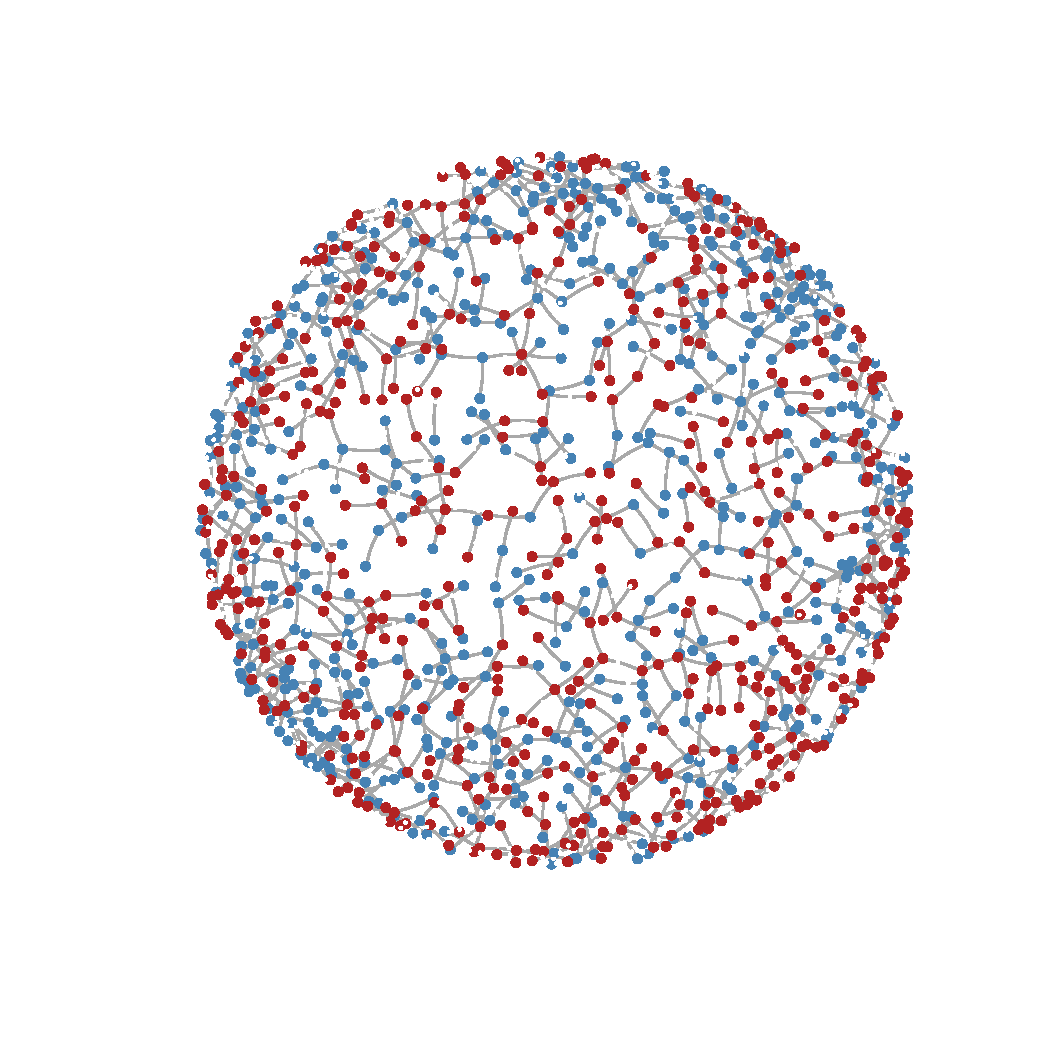
\includegraphics[trim={2cm 2cm 2cm 2cm}, clip, width=\linewidth]{draft/network_plots1.pdf} 
        \caption*{A. Erdos-Renyi random network}
        \label{fig1:random}
    \end{subfigure}
    \hfill
    \begin{subfigure}[t]{0.45\textwidth}
        \centering
        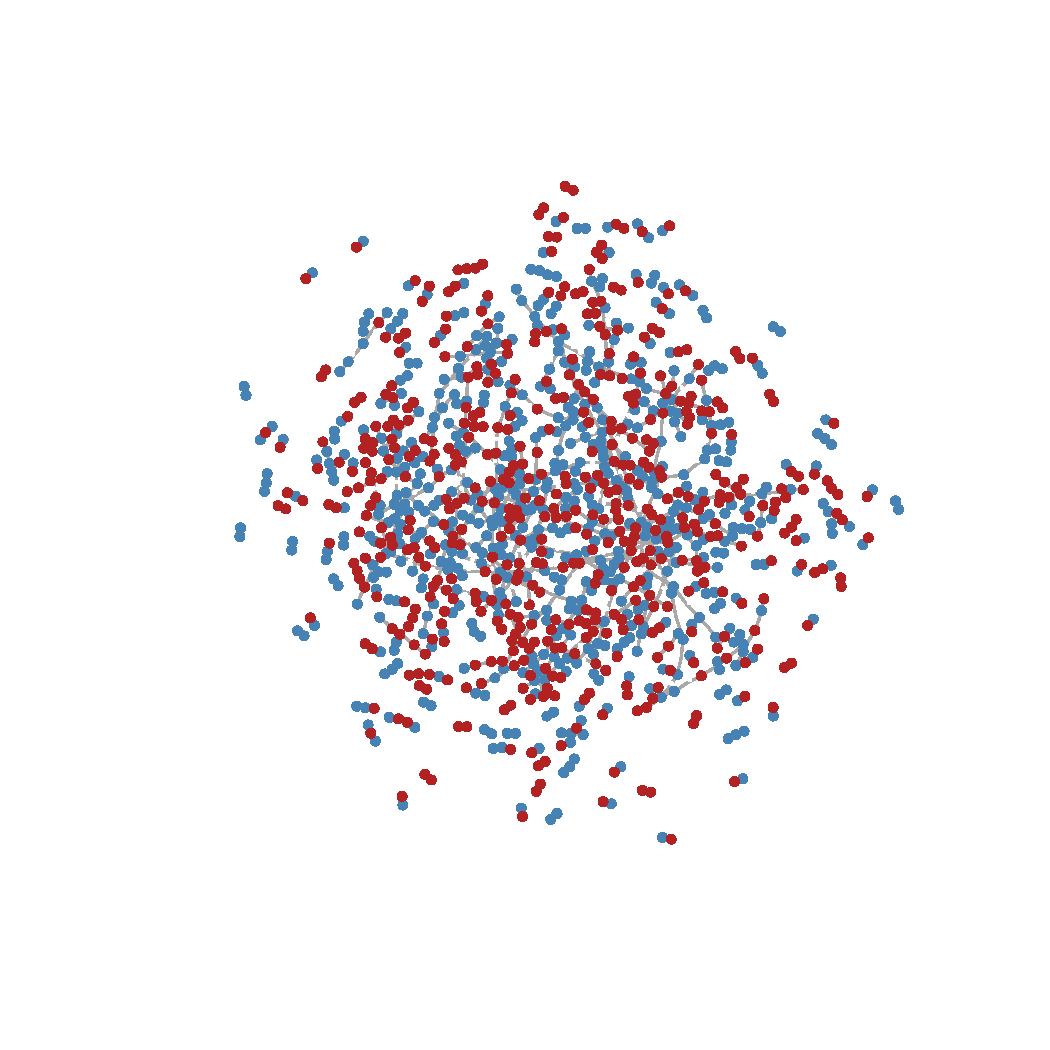
\includegraphics[trim={2cm 2cm 2cm 2cm}, clip, width=\linewidth]{draft/network_plots2.pdf} 
        \caption*{B. Chain network} \label{fig1:tree}
    \end{subfigure}

    \vspace{1cm}
    \begin{subfigure}[t]{0.45\textwidth}
        \centering
        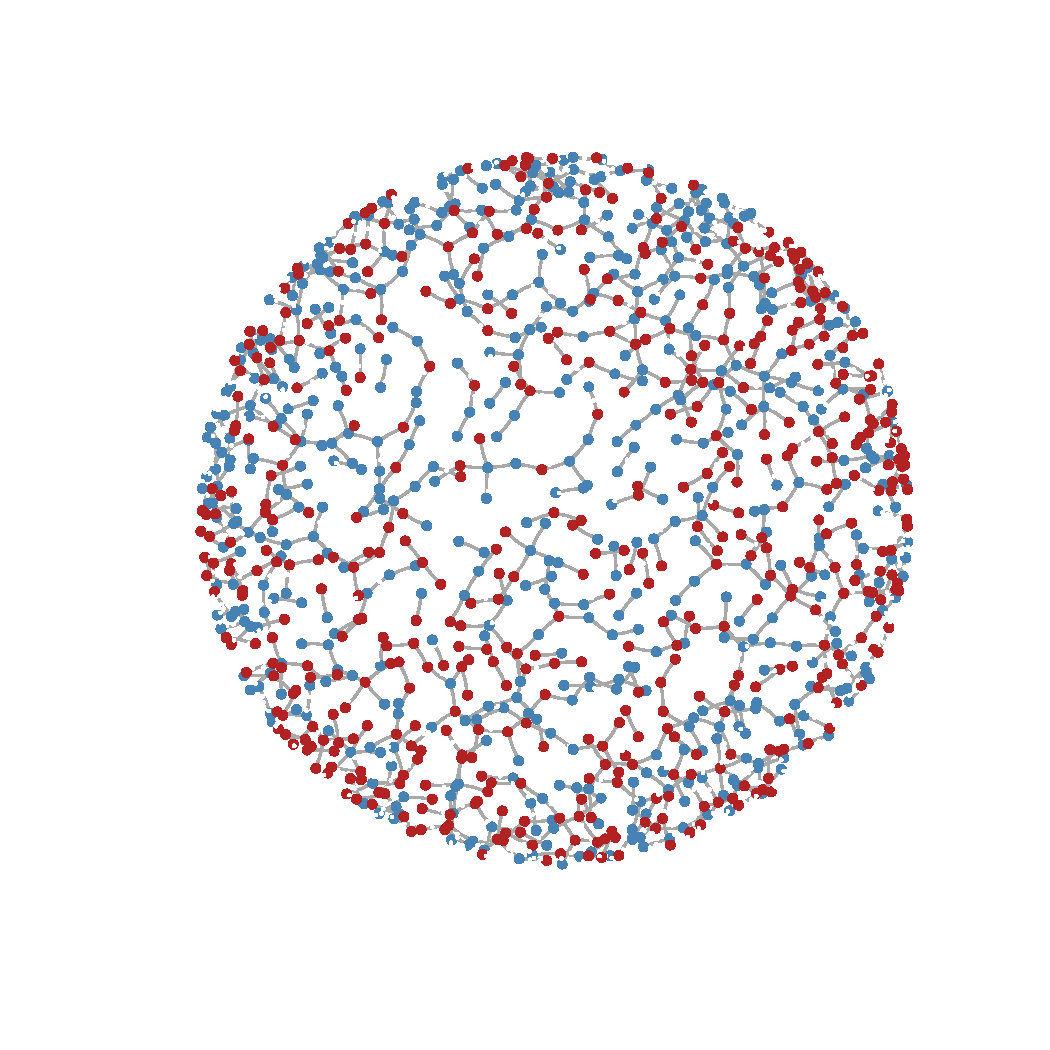
\includegraphics[trim={2cm 2cm 2cm 2cm}, clip, width=\linewidth]{draft/network_plots3.pdf} 
        \caption*{C. Small-world network absent homophily} \label{fig1:nohomophily}
    \end{subfigure}
    \hfill
    \begin{subfigure}[t]{0.45\textwidth}
        \centering
        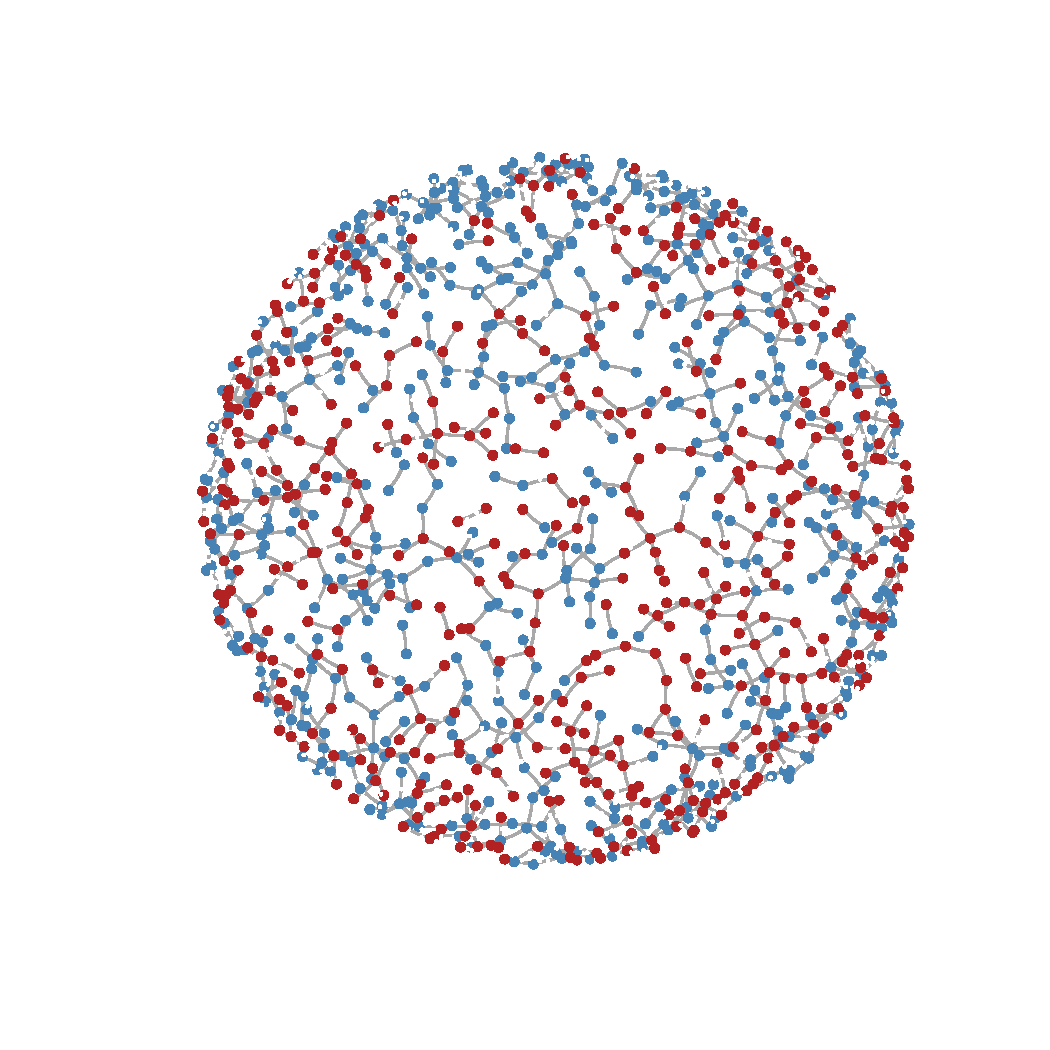
\includegraphics[trim={2cm 2cm 2cm 2cm}, clip, width=\linewidth]{draft/network_plots4.pdf} 
        \caption*{D. Baseline small-world network} \label{fig1:smallworld}
    \end{subfigure}
    
    \vspace{1cm}
    \captionsetup{format=hang}
    \caption{A cross-sectional view of simulated networks from different network topologies.} 
    \label{fig:Figure1}
    \captionsetup{font=small}
    \caption*{Note: Colored nodes represent nodes that have at least one connection with their neighbor (Red = Republicans, Blue = Democrats) while isolates at given time point was suppressed in visualization. A Erdos-Renyi (ER) random network ( = A) assumes a homogeneous probability of creating and dropping ties across all nodes conditional on observed density. A chain-like network ( = B) has more longer chains than the ER random network while lacks triangle-like structure due to constrains on degrees (less than three). While two small-world network has more star-like structure than others, our baseline small-world network (= D) is more homophilous than competing specification in its counterpart without homophily (= C), as can be seen in Table \ref{tab:Table1}.} 
\end{figure}    

  Adapting a well-known class of epidemic models, we simulated the dynamics of misinformation exposure and its correction on top of those stochastic network evolution models. We setup an environment consist of 2400 partisan actors (based on 2009 ANES panel survey's partisan composition: see footnote \ref{note6} for a detail) and simulate the diffusion dynamics over 1000 simulated hours (roughly corresponds to 41 days) with 100 replicated simulations per scenario. We fit a series of SEIR (\enquote{susceptible - exposed - infected - recovered}) dynamic models for (a) a simple contagion of misinformation (i.e., a progression from \enquote{suspected} to \enquote{exposed}), (b) a progression from \enquote{exposed} to \enquote{infected} (i.e., those who believe a given misinformation conditional on exposure), and (c) a progression from \enquote{infected} to \enquote{recovered} conditional on adoption of corrective messages from their peers following complex contagion logics. 

\subsection{Misinformation Transmission}
    
    To date, how many times people exactly \enquote{share} fake news and misinformation on their social networks is not yet well known to public. However, a recent study by \citeauthor{allcott2017social} (\citeyear{allcott2017social}) report that, for all 65 fake news websites they have identified during 2016 election, an individual visited such sites 0.64 times on average, and among them 41.8\% of all visits originate from social media traffics. Similarly, \citeauthor{guess2018selective} (\citeyear{guess2018selective}) report that of 27.4\% individuals who visited fake news websites, 22.1\% of all visits originate from social media. 

  We start by setting our baseline prevalence, of which we arbitrary set 15\% of partisans are initially affected by misinformation and fake news. We then set our baseline \enquote{act rate} (i.e., the average number of transmissible acts per unit time per discussion tie) by taking the average of estimates from \citeauthor{allcott2017social} (\citeyear{allcott2017social}) and from \citeauthor{guess2018selective} (\citeyear{guess2018selective}), which yields 0.164 times per hour per discussion tie.\footnote{ \citeauthor{allcott2017social} report 0.64 $\times$ 41.8\% = 0.268 shares per unit time, while \citeauthor{guess2018selective} report 0.274 $\times$ 22.1\% = 0.060 shares per unit time. This averages to 0.164 times per unit time. We additionally assume all fake news website visits are driven by information sharing on social media.} We further assume 15\% of those who initially affected are only Republicans, given that the vast majority of identified fake news articles during 2016 U.S. presidential election were overwhelmingly pro-Trump \parencite[e.g.,][]{guess2018selective}. Here, we assume misinformation ``always'' flows from the \enquote{infected} (i.e., those who believe given misinformation) to their susceptible peers (i.e., those who are not yet exposed), but those who are being merely exposed do not contribute to misinformation flow (since the mere exposure does not necessarily mean they are endorsing such information) nor any other sources of exposure to misinformation is possible (i.e., partisan media exposure) for an individual to encounter such misinformation. 
    
    Progression from \emph{being susceptible} (i.e., not yet being exposed) to \emph{being exposed} was determined by a simple contagion, such that a single contact with those who are infected ( = threshold value of 1) is sufficient for partisans to be exposed to misinformation, yet conditional on the propensity for those who are infected to actually share such news (i.e., the probability of infection: see below). Following PEW data \parencite{pewfakenews} which suggests approximately 16\% of all partisans have had \emph{shared} fake news stories on their social network, we assume the risk of transmission of those who are already infected to share misinformation (i.e., infection probability per act) to be .16 in our simulations. Combining those two parameters for the probability of infection per act (= .16) and the number of acts per unit time (= .164), the per-discussion tie transmission rate is calculated as an exponential function of the two, with a Bernoulli probability distribution controlling whether an infection event occurs stochastically. In addition, we additionally assume Republicans on average have a higher infection probability per act than Democrats (= .04 higher than Democrats) -- once infected, Republicans are more likely to share such news than Democrats -- given the directional nature of misinformation being considered within this context (e.g., the vast majority of fake news articles during 2016 U.S. presidential election were overwhelmingly pro-Republican).
    
\subsection{Progression from Exposed to Infectious States}
    Progression from \emph{being exposed} to \emph{being infected} (i.e., transition between exposed to infectious states) was modeled as individual-level stochastic processes, in which there is a differential hazard of transition across partisans following a Bernoulli distribution with the transition rate parameter. Consistent with partisan motivated reasoning accounts \parencite{taber2006, nyhan2010corrections}, we set Republicans to have higher transition rates overall (= .30) than Democrats (= .07) given pro-republican misinformation exposure when they are at their mean level of accuracy motivations, where accuracy motivations are assumed to be normally distributed among population. We set these rate parameters based on results reported in \citeauthor{garrett2016driving} (\citeyear{garrett2016driving}), where they show that online partisan news use increases the chance of incorrectly answering the given factual knowledge question by approximately 30\% points for Republicans and 7\% point for Democrats compared to those who do not exposed to such information (see their Table S6 for a detail). Also, we assume those who score high in their accuracy motivations to have a lower transition rate regardless of their partisanship (see the online appendix for a detail), effectively treating one's partisanship and accuracy motivations as individual-level moderators of misinformation adoption process. 

\subsection{Corrective Message Exposure and a Recovery from Misperceptions}
  For corrective message exposure and subsequent progression from \emph{being infected} to \emph{being recovered}, we examine two possible scenarios -- the first model closely approximate a single-shot, \emph{asocial} correction, in that the model assumes  corrections are randomly received for infected individuals, following individual-level stochastic process of adopting such corrections given exposure. This model therefore assumes no social-dynamics surrounding the misinformation correction, as typically assumed in extant experimental literature. Our second, more realistic model is more consistent with our prior discussion of simple vs. complex contagion dynamics, in that once exposed, individuals progress to recovery state when a certain proportion (= $\rho$) of his or her neighbors are sending corrective messages that debunking misinformation. In these scenarios, we assume approximately half of one's immediate neighbors (\enquote{alters}) who are not yet affected and/or already being recovered from misinformation send correction messages to the infected ego. We systematically vary the threshold value of $\rho$ to explore system-level consequences of social dynamics surrounding misinformation corrections. Below Table \ref{tab:Table2} lists all scenarios for the combination of network topological structure and the threshold value of $\rho$ in misperception recovery. 
\centerline{ -- Table \ref{tab:Table2} about here -- }  

\section{Results}
\subsection{Simple Contagions of Misinformation Exposure}
  We first look at the simple contagion dynamics of misinformation exposure (assuming no recovery by corrections throughout the simulated time periods) and propagation rates across different network typologies over time, as depicted in Figure \ref{fig:Figure2} and in Table \ref{tab:Table3} below. The results reveal that network structures have somewhat non-trivial effects on the dynamics of misinformation propagation at population level. It seems that our baseline network model (i.e., small-world network with partisan homophily) appears to be bit better in terms of disseminating given misinformation more faster than other network structures -- that is, we do find some modest evidence that spread of simple misinformation spreads faster in our small world networks (red lines in Panel A of Figure \ref{fig:Figure2}) than in random networks (black lines in Panel A of Figure \ref{fig:Figure2}) when misinformation is spread via simple contagion (i.e., a single contact with those who are infected) followed by a individual-level stochastic progression to being infected given exposure to misinformation. 
\centerline{ -- Table \ref{tab:Table3} and Figure \ref{fig:Figure2} about here -- }  

    Although differences among the cumulative exposure fractions in different network structures were not appear to be vastly different from each other (as their confidence intervals of cumulative exposure fractions significantly overlap with each other: see online supplementary materials for a detail), their exposure rates (as measured by the number of newly exposed individuals at given time point) do differ with each other as can be seen in Figure \ref{fig:Figure2} below. This was especially true between our baseline network (red lines) and random networks (black lines) as indicated in Table \ref{tab:Table4}. We used the Wilcoxon Rank Sum Test (a nonparametric test of differences of two population distributions) to test whether the two proportions of newly exposed to misinformation among the susceptible (= no. of SI flow divided by no. of susceptible per each time point) significantly differ from each other between different network topologies. The cell entries of Table \ref{tab:Table4} refer to the range of simulated time points in which two distributions of adoption rates statistically different from each other based on Wilcoxon Rank Sum Test. For instance, Table \ref{tab:Table4} indicates that from 58 to 901 time points, the distribution of the fraction of newly exposed to misinformation from ER random network and that from our baseline small-world homophily network statistically different from zero (less than .05). The results shows that across range of time points excluding the very initial stage of misinformation propagation, network structure induces statistically different adoption rates over time.    
\centerline{ -- Table \ref{tab:Table4} about here -- }  

\begin{figure}
\captionsetup[figure]{labelfont={bf,it}}
    \centering
    
    \begin{subfigure}[t]{0.8\textwidth}
        \centering
        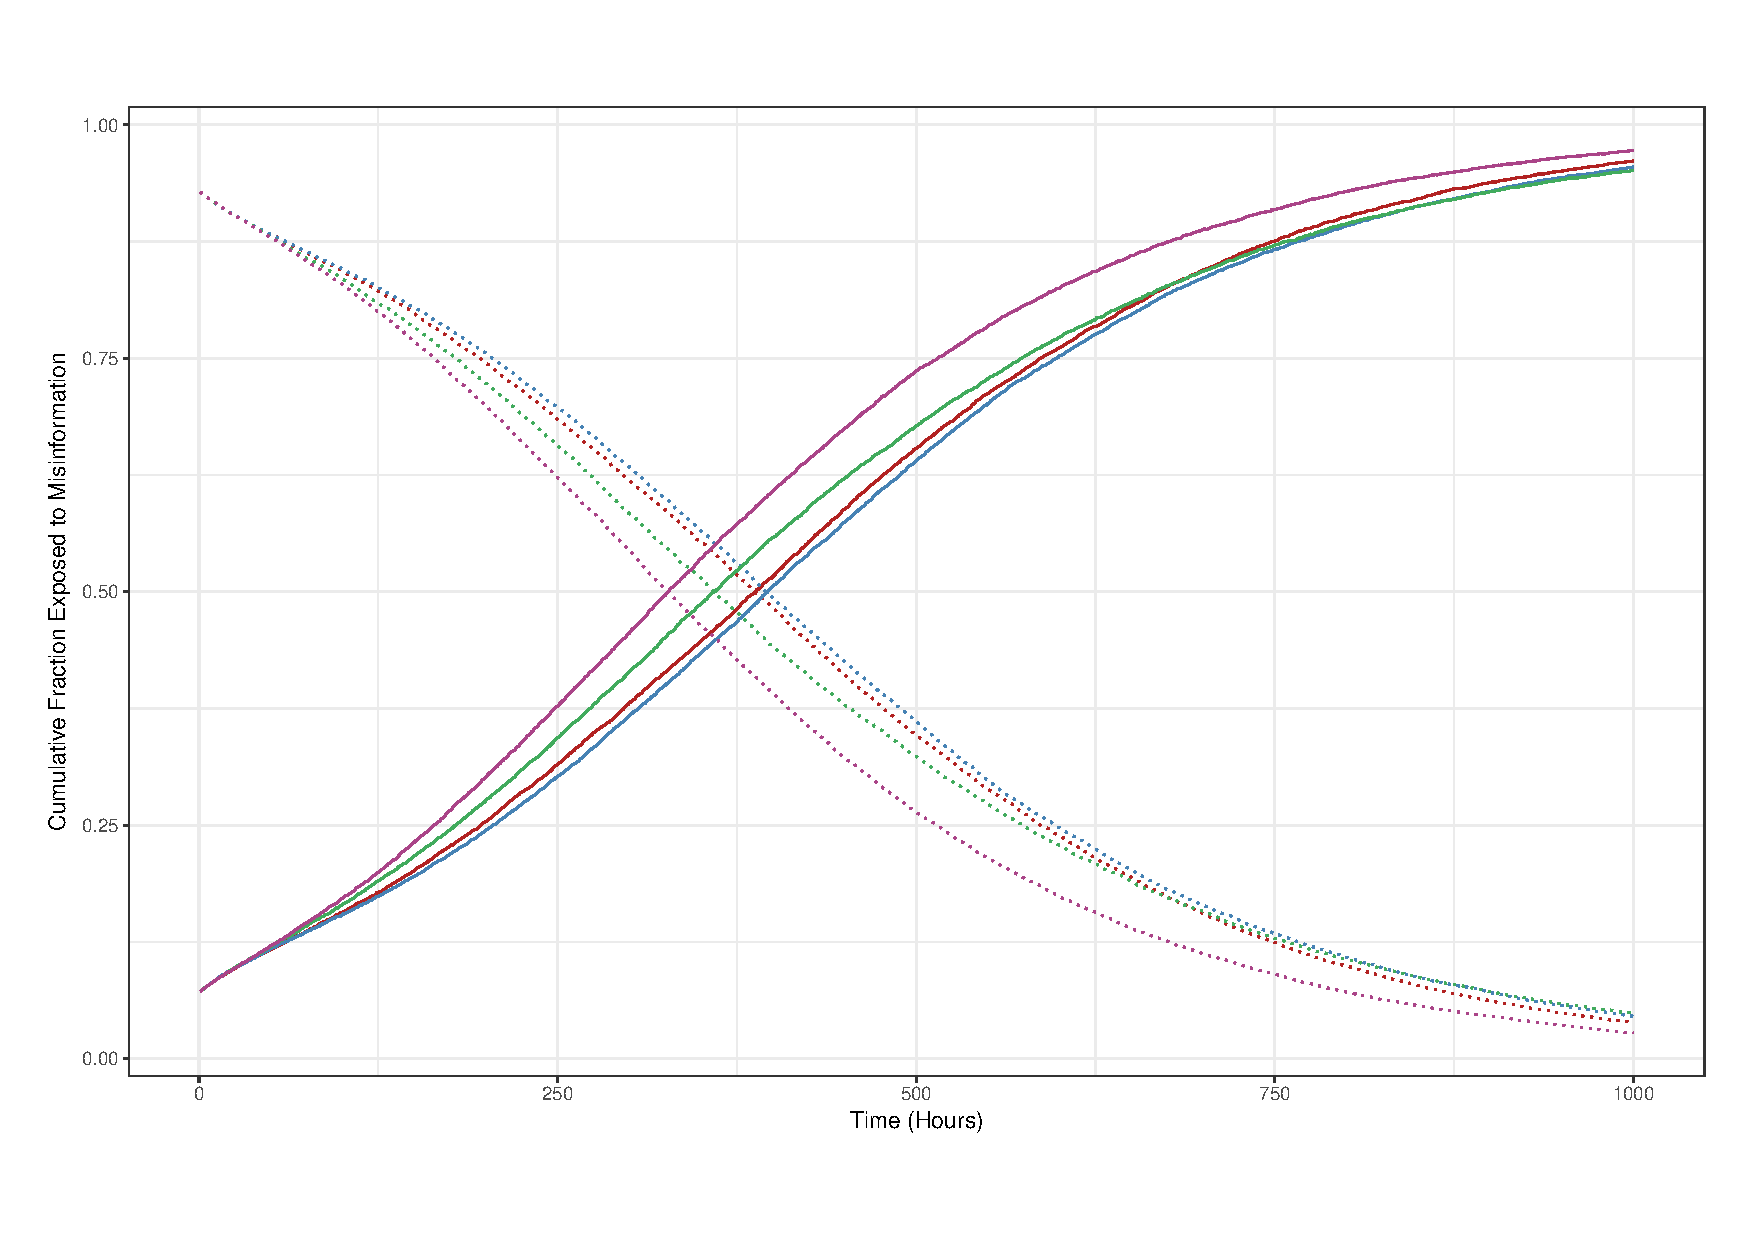
\includegraphics[clip, width=\linewidth, page = 1]{draft/Figure_2__Prevalence.pdf} 
        \captionsetup{font=small}
        \caption*{Panel A. Overall Cumulative Prevalence of Misinformation.}
    \end{subfigure}
  
    \begin{subfigure}[t]{0.8\textwidth}
        \centering
        \includegraphics[clip, width=\linewidth, page = 2]{draft/Figure_2__Prevalence.pdf} 
        \captionsetup{font=small}
        \caption*{Panel B. Incidence Rates of New Exposure to Misinformation (the number of newly exposed to misinformation)}
    \end{subfigure}
    
    \captionsetup{format=hang}
    \caption{Prevalence and Incidence Rates of Misinformation Over Time by Network Topologies (Assuming No Recoveries, Averaged Over 100 Simulations).} 
    \label{fig:Figure2}
    \captionsetup{font=small}
    \caption*{Note: Straight lines in Panel A represent fraction of those who are being exposed to misinformation, whereas dotted lines represent fraction of those who are susceptible. X-axis represents simulated times (in hours) and Y-axis represents the fraction exposed to misinformation (in panel A) or rates of misinformation exposure (in panel B). Red = Erdos-Renyi random network, Blue = Chain network, Green = Small-world absent homophily, and Violet = baseline small-world homophily network.} 
\end{figure}          
        
% Table 3 and Table 4
\begin{table}[!htbp] 
  \begin{minipage}{\textwidth}
    \centering
  \caption{\\ Misinformation Exposure Prevalence Per 100 Individuals Over Time by Network Topologies (Cumulative Exposure, No Recovery Scenarios)} 
  \label{tab:Table3} 
\begin{tabular}{@{\extracolsep{5pt}} ccccc} 
\\[-1.8ex]\hline 
\hline \\[-1.8ex] 
 & \textbf{E-R} & \textbf{Chain} & \textbf{SW No-Homophily} & \textbf{SW Homophily} \\ 
\hline \\[-1.8ex] 
\textbf{Overall} & .594 & .584 & .605 & .640 \\ 
(95\% CIs) & [.564, .624] & [.558, .609] & [.574, .635] & [.608, .669] \\ 
\hdashline
\textbf{Among Dem} & .295 & .290 & .301 & .312 \\ 
(95\% CIs) & [.274, .316] & [.271, .308] & [.279, .322] & [.287, .332] \\ 
\hdashline
\textbf{Among Rep} & .299 & .295 & .305 & .330 \\ 
(95\% CIs) & [.285, .313] & [.282, .307] & [.290, .319] & [.315, .343] \\ 
\hline \\[-1.8ex] 
\end{tabular} 
\begin{tablenotes}[para,flushleft]
\small \vspace{0.15in}
\textbf{Note:} E-R: Erdos Renyi random network. Chain: Chain network. SW No-Homophily: Small-world network absent of homophily. SW Homophily: Small-world network with partisan homophily. All statistics are based on 100 random simulations over 1000 time points from the same setup per network topologies. \\ 
\end{tablenotes}
\end{minipage}
\bigbreak
\vspace{0.5in}
  \begin{minipage}{\textwidth}
    \centering
  \caption{\\Time Durations Within Which WRS Test of Differences on Fraction of Newly Exposed of Misinformation Over Time are Significantly Different From Each Other Across Topologies} 
  \label{tab:Table4} 
  \begin{tabular}{@{\extracolsep{5pt}} ccccc} 
\\[-1.8ex]\hline 
\hline \\[-1.8ex] 
 & \textbf{E-R} & \textbf{Chain} & \textbf{SW No-Homophily} & \textbf{SW Homophily} \\ 
\hline \\[-1.8ex] 
\textbf{Chain} & 106 : 278 & - &  &  \\ 
\textbf{SW No-Homophily} &  68 : 1000 &  70 : 585 & - &  \\ 
\textbf{SW Homophily} &  58 : 901 &  63 : 942 & 151 : 1000 & - \\ 
\hline \\[-1.8ex] 
\end{tabular} 
\begin{tablenotes}[para,flushleft]
\small \vspace{0.15in}
\textbf{Note:} E-R: Erdos Renyi random network. Chain: Chain network. SW No-Homophily: Small-world network absent of homophily. SW Homophily: Small-world network with partisan homophily. Cell entries denote the range of time points in which Wilcoxon Rank Sum test indicates the adoption rates from two network topologies statistically different from each other (p < 0.05). \\ 
\end{tablenotes}
\end{minipage}
\end{table} 


\subsection{Complex Contagions of Misinformation Corrections}
  We now examine complex contagion dynamics of corrective message adoption and its impacts on population-level dynamics of misinformation propagation (detailed recovery scenarios are described in Table \ref{tab:Table2}). Table \ref{tab:Table5} lists results for all scenarios in terms of prevalence of misinformation and number of those who are newly being recovered per hour, and Panel A to Panel D in Figure \ref{fig:Figure3} graphically depicts these results.  
\centerline{ -- Table \ref{tab:Table5} and Figure \ref{fig:Figure3} about here -- }     
    
% Table 5    
\begin{sidewaystable}[ht]
  \centering
    \caption{\\ Asocial vs. Thresholds Recovery Model Results} 
  \label{tab:Table5} 
\begin{tabular}{cccccc}
 \toprule
       \multicolumn{1}{c}{} &  \multicolumn{1}{c}{} & 
      \multicolumn{1}{c}{Scenario I} &
      \multicolumn{3}{c}{Scenario II - Thresholds} \\
\cline{4-6}
 &   & \textbf{Asocial} & \textbf{0.25} & \textbf{0.5} & \textbf{0.75} \\
  \midrule
               \textbf{E-R} & I Prevalence & 23.484 [20.663, 26.037] & 3.661 [3.070, 4.406] & 3.722 [3.031, 4.503] & 5.398 [4.383, 6.844] \\ 
                            & R Incidence & 1.262 [.000, 3.716] & .429 [.150, 1.350] & .423 [.130, 1.383] & .520 [.0433, 1.944] \\ 
             \textbf{Chain} & I Prevalence & 22.746 [20.051, 25.492] & 3.581 [2.983, 4.286] & 3.581 [2.983, 4.286] & 5.260 [4.259, 6.399] \\ 
                            & R Incidence & 1.196 [.000, 3.625] & .405 [0.138, 1.339] & .405 [0.138, 1.339] & .483 [.0372, 1.843] \\ 
   \textbf{SW No-Homophily} & I Prevalence & 24.107 [21.220, 27.047] & 3.926 [3.266, 4.693] & 4.016 [3.347, 4.821] & 6.107 [4.951, 7.639] \\ 
                  & R Incidence & 1.329 [.000, 3.797] & .452 [.176, 1.465] & .457 [.150, 1.483] & .599 [.050, 2.150] \\ 
      \textbf{SW Homophily} & I Prevalence & 26.039 [23.029, 29.007] & 3.863 [3.148, 4.724] & 3.983 [3.295, 4.884] & 6.014 [4.935, 7.423] \\ 
                  & R Incidence & 1.420 [.003, 4.003] & .495 [.188, 1.461] & .494 [.168, 1.508] & .656 [.0771, 2.127] \\ 
   \bottomrule
\end{tabular}
\begin{tablenotes}[para,flushleft]
\small \vspace{0.15in}
\textbf{Note:} E-R: Erdos Renyi random network. Chain: Chain network. SW No-Homophily: Small-world network absent of homophily. SW Homophily: Small-world network with partisan homophily. I Prevalence: Infection prevalence per 100 individuals over time. R Incidence: Recovery incidence per time. \\ 
\end{tablenotes}
\end{sidewaystable} 

% Figure 3
\begin{sidewaysfigure}
\captionsetup[figure]{labelfont={bf,it}}
\captionsetup[subfigure]{labelfont=bf,textfont=normalfont,singlelinecheck=on}
    \centering
    \begin{subfigure}[t]{0.49\textwidth}
        \centering
        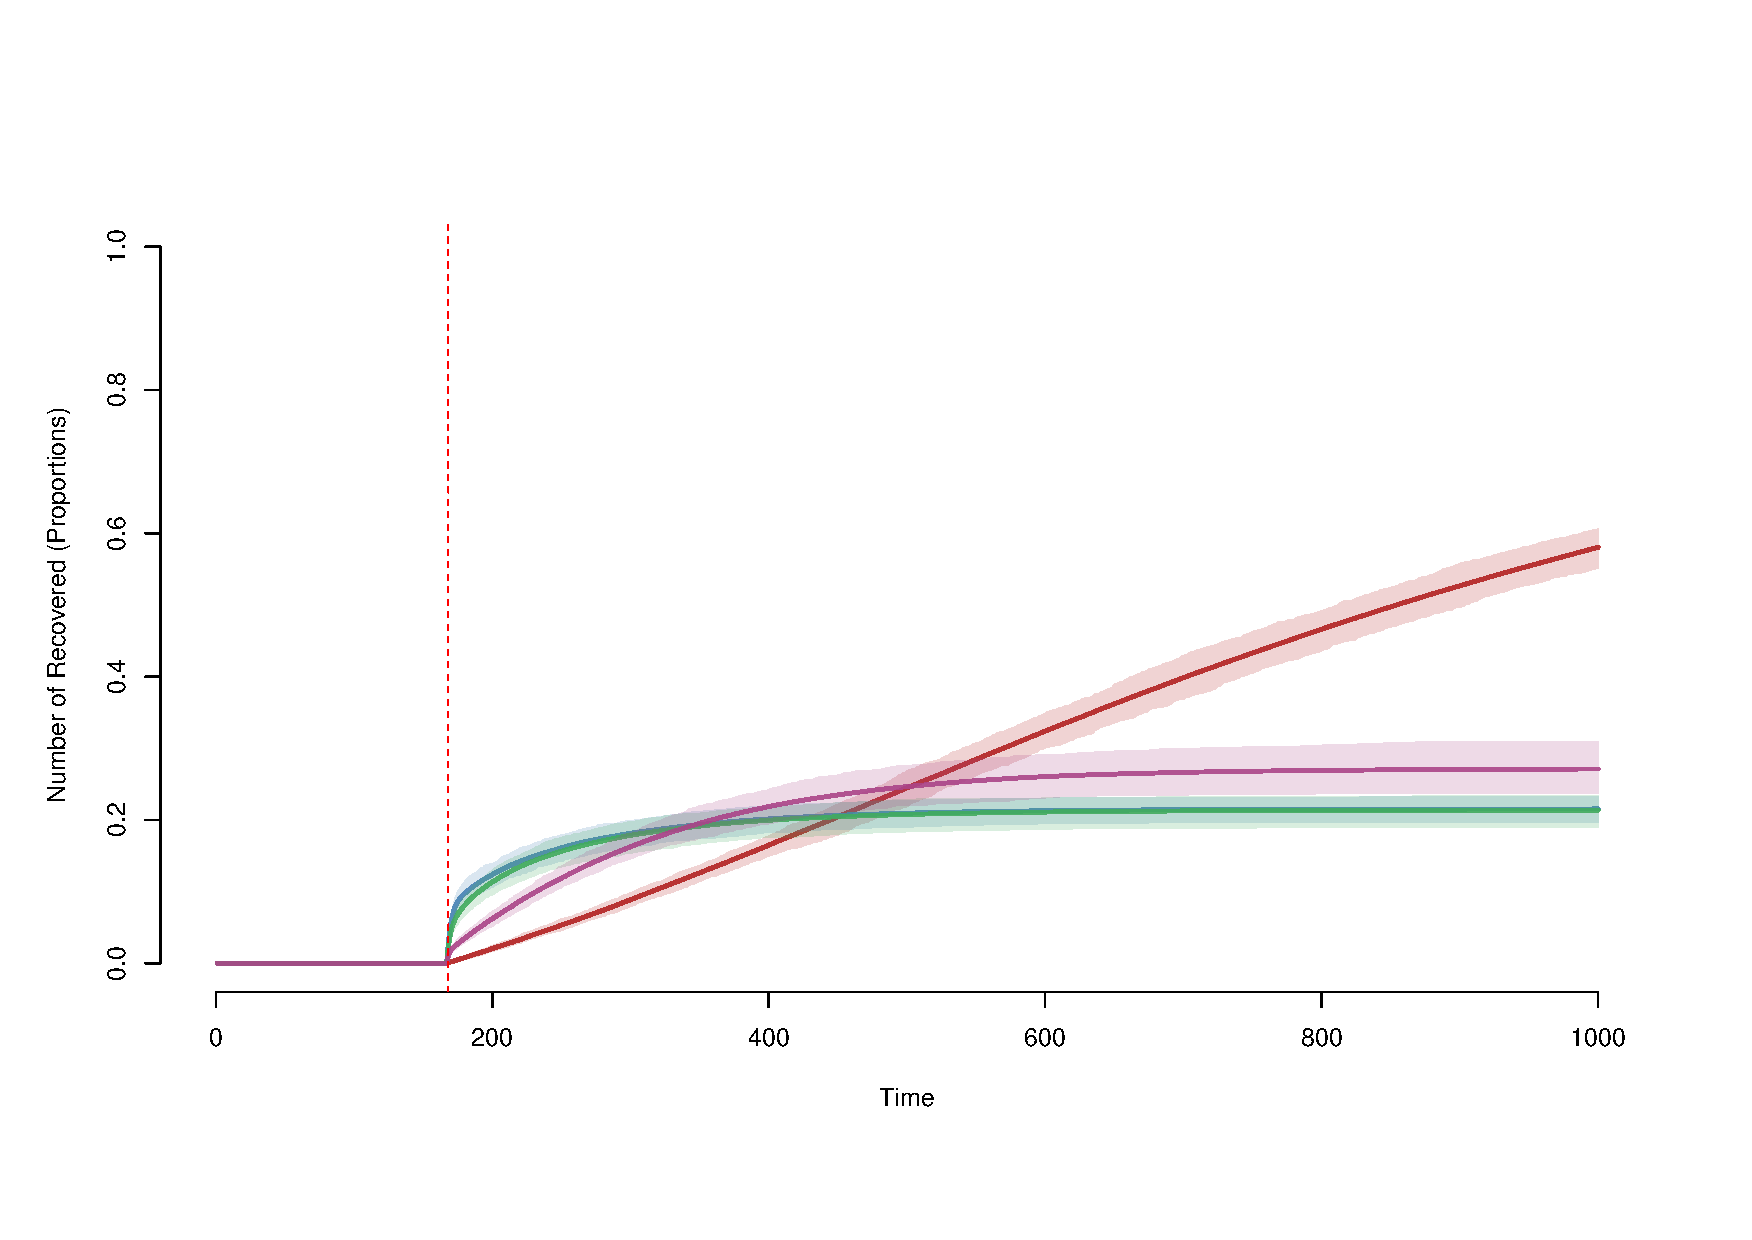
\includegraphics[trim={1.5cm 2.7cm 2cm 5cm}, clip, width=\linewidth]{draft/Fig3a.pdf} 
        \caption*{A. Erdos-Renyi random network}
        \label{fig3:random}
    \end{subfigure}
    \hfill
    \begin{subfigure}[t]{0.49\textwidth}
        \centering
        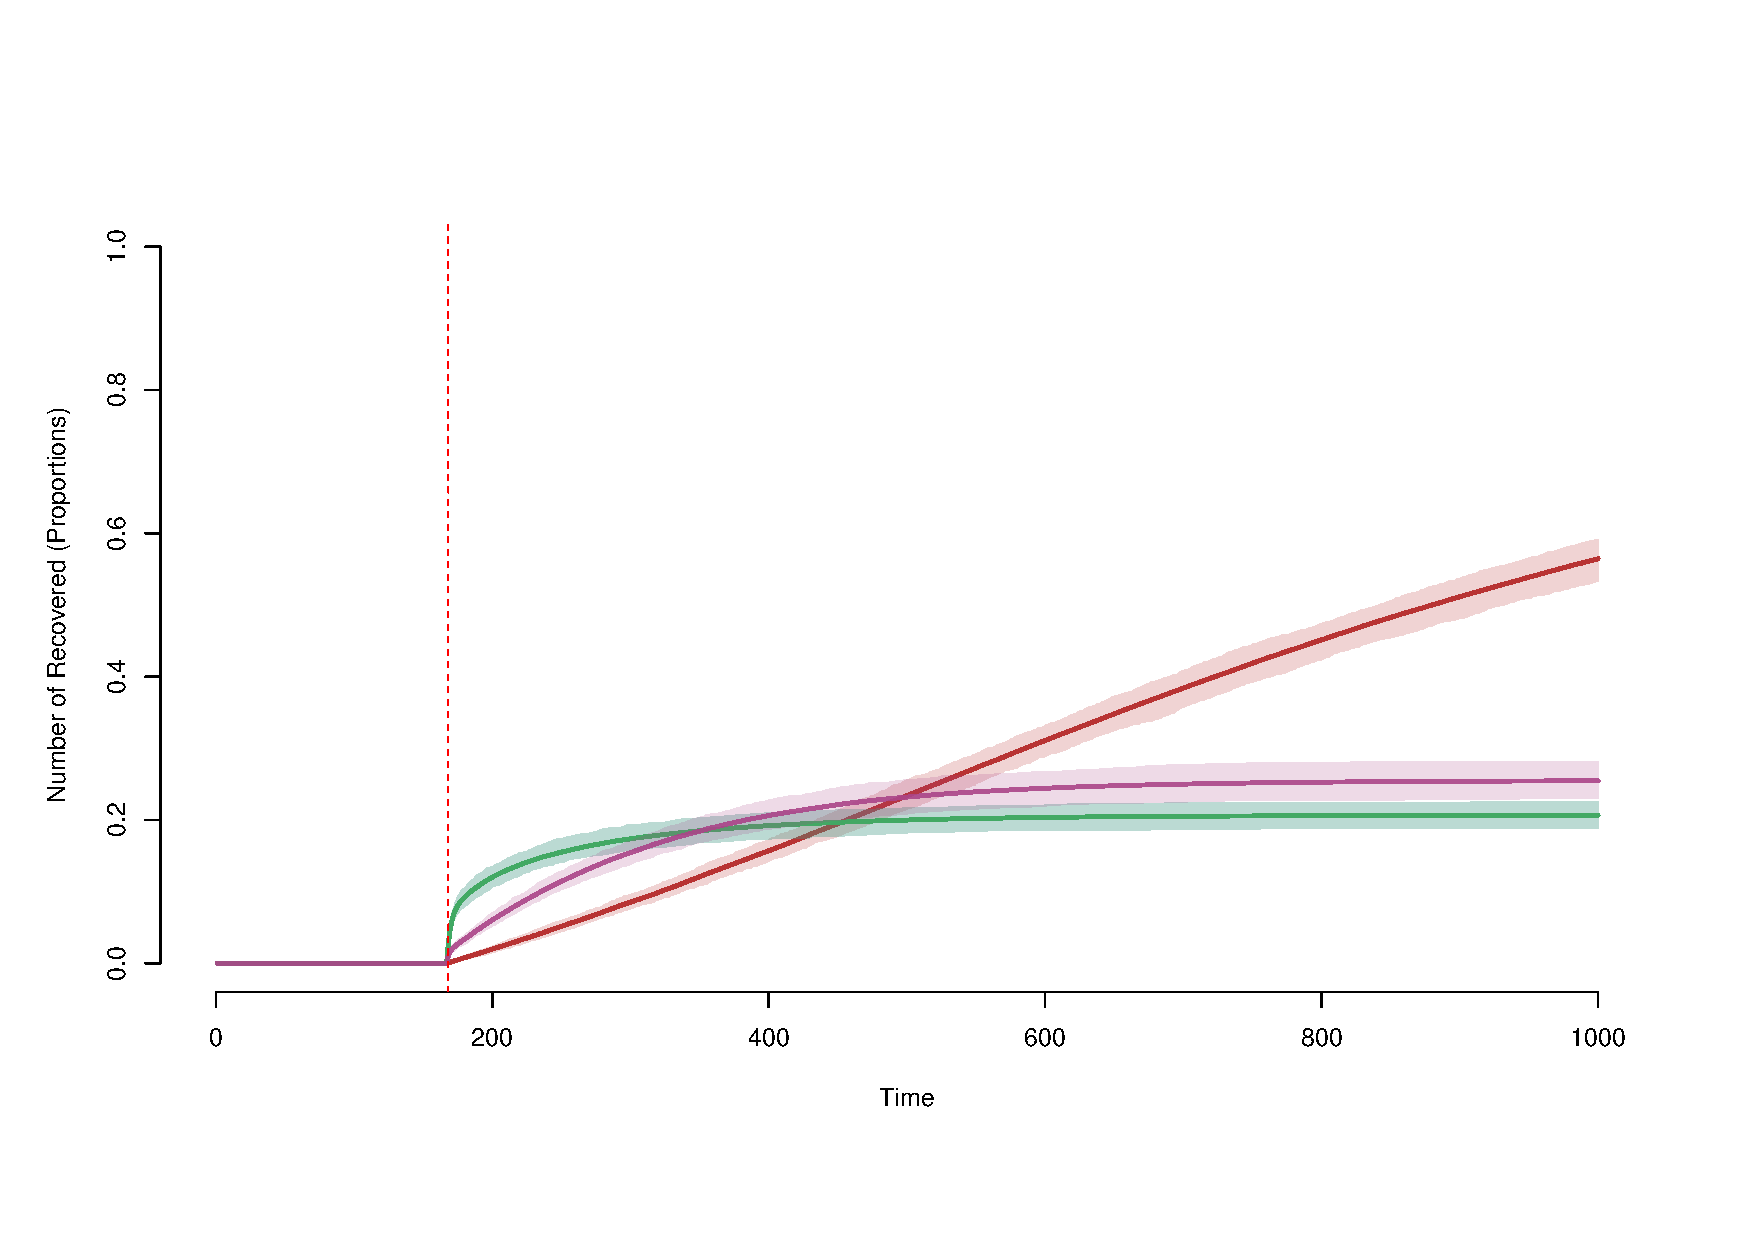
\includegraphics[trim={1.5cm 2.7cm 2cm 5cm}, clip, width=\linewidth]{draft/Fig3b.pdf} 
        \caption*{B. Chain network} \label{fig3:chain}
    \end{subfigure}

    \vspace{1cm}
    \begin{subfigure}[t]{0.49\textwidth}
        \centering
        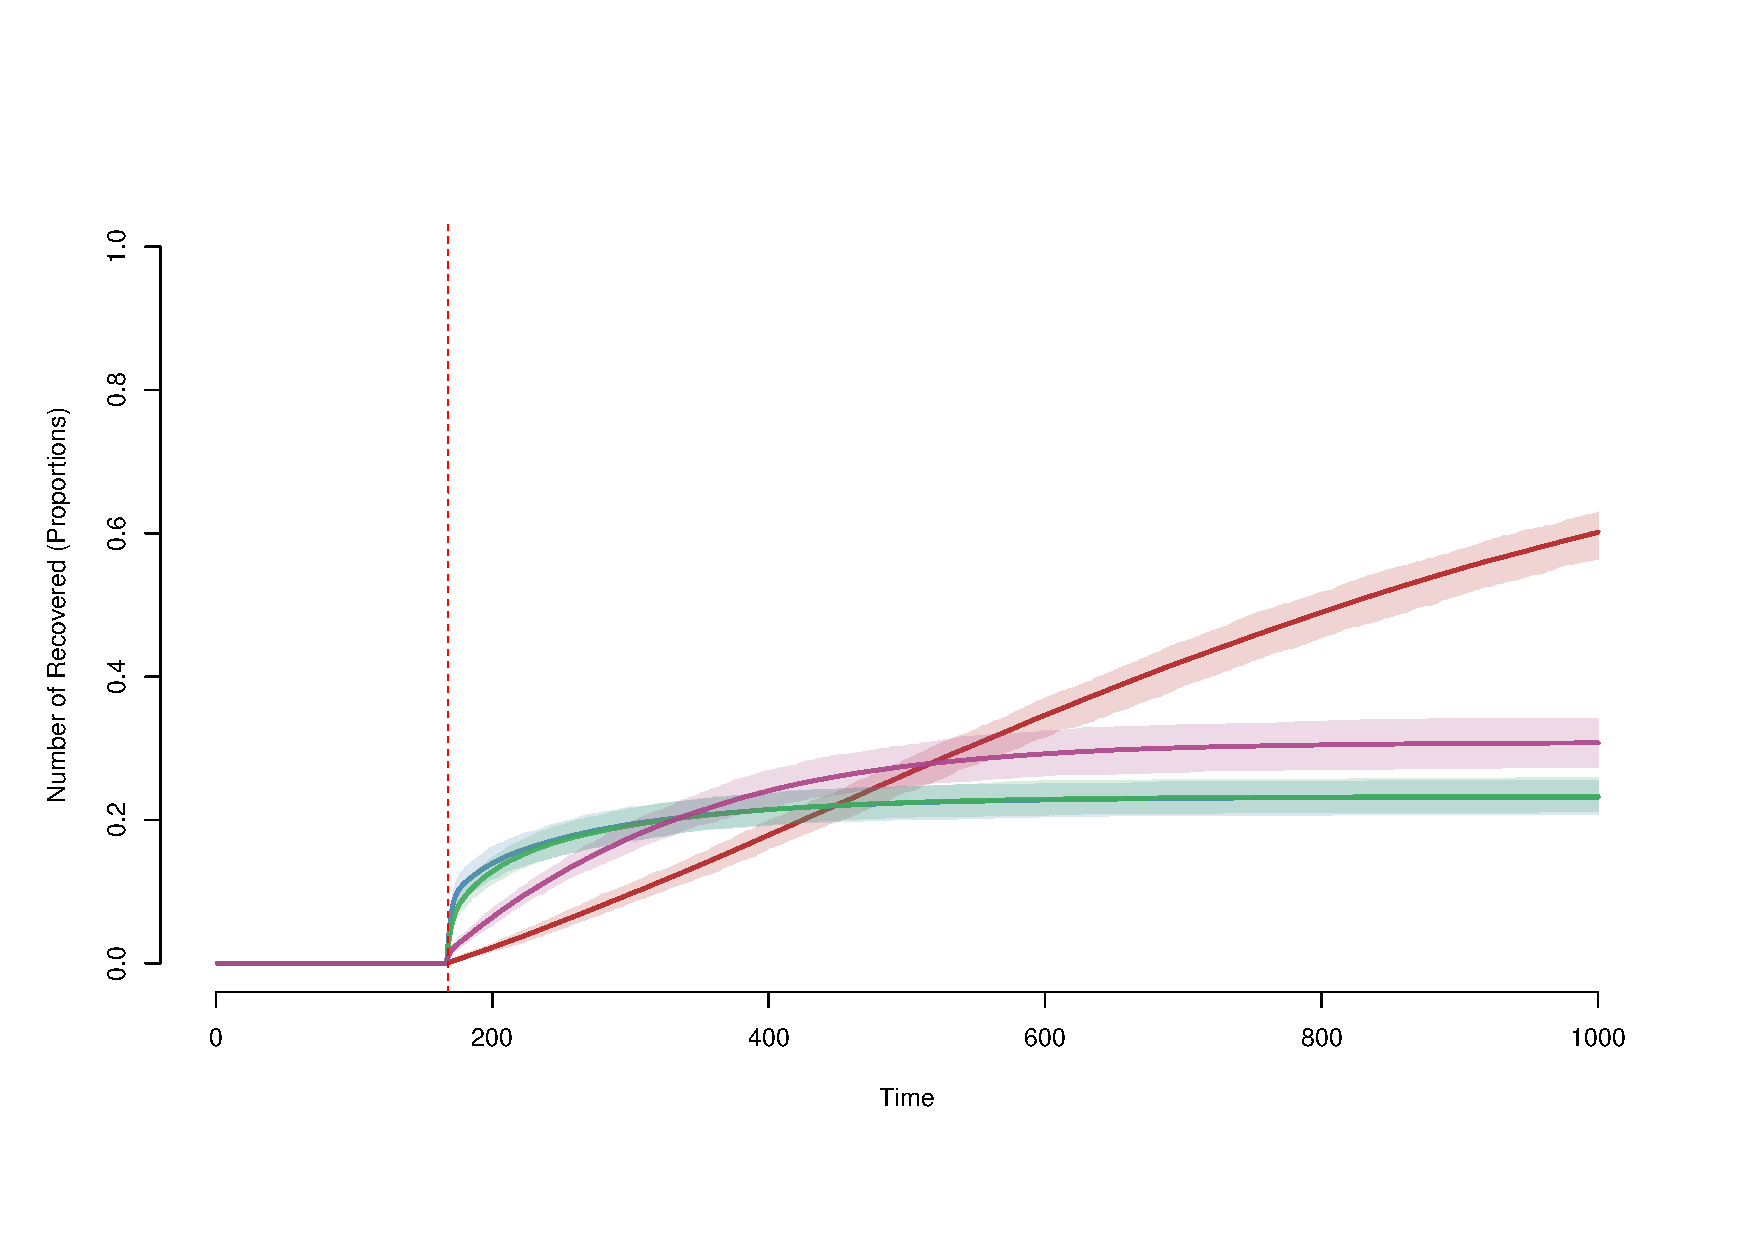
\includegraphics[trim={1.5cm 2.7cm 2cm 5cm}, clip, width=\linewidth]{draft/Fig3c.pdf} 
        \caption*{C. Small-world network absent homophily} \label{fig3:nohomophily}
    \end{subfigure}
    \hfill
    \begin{subfigure}[t]{0.49\textwidth}
        \centering
        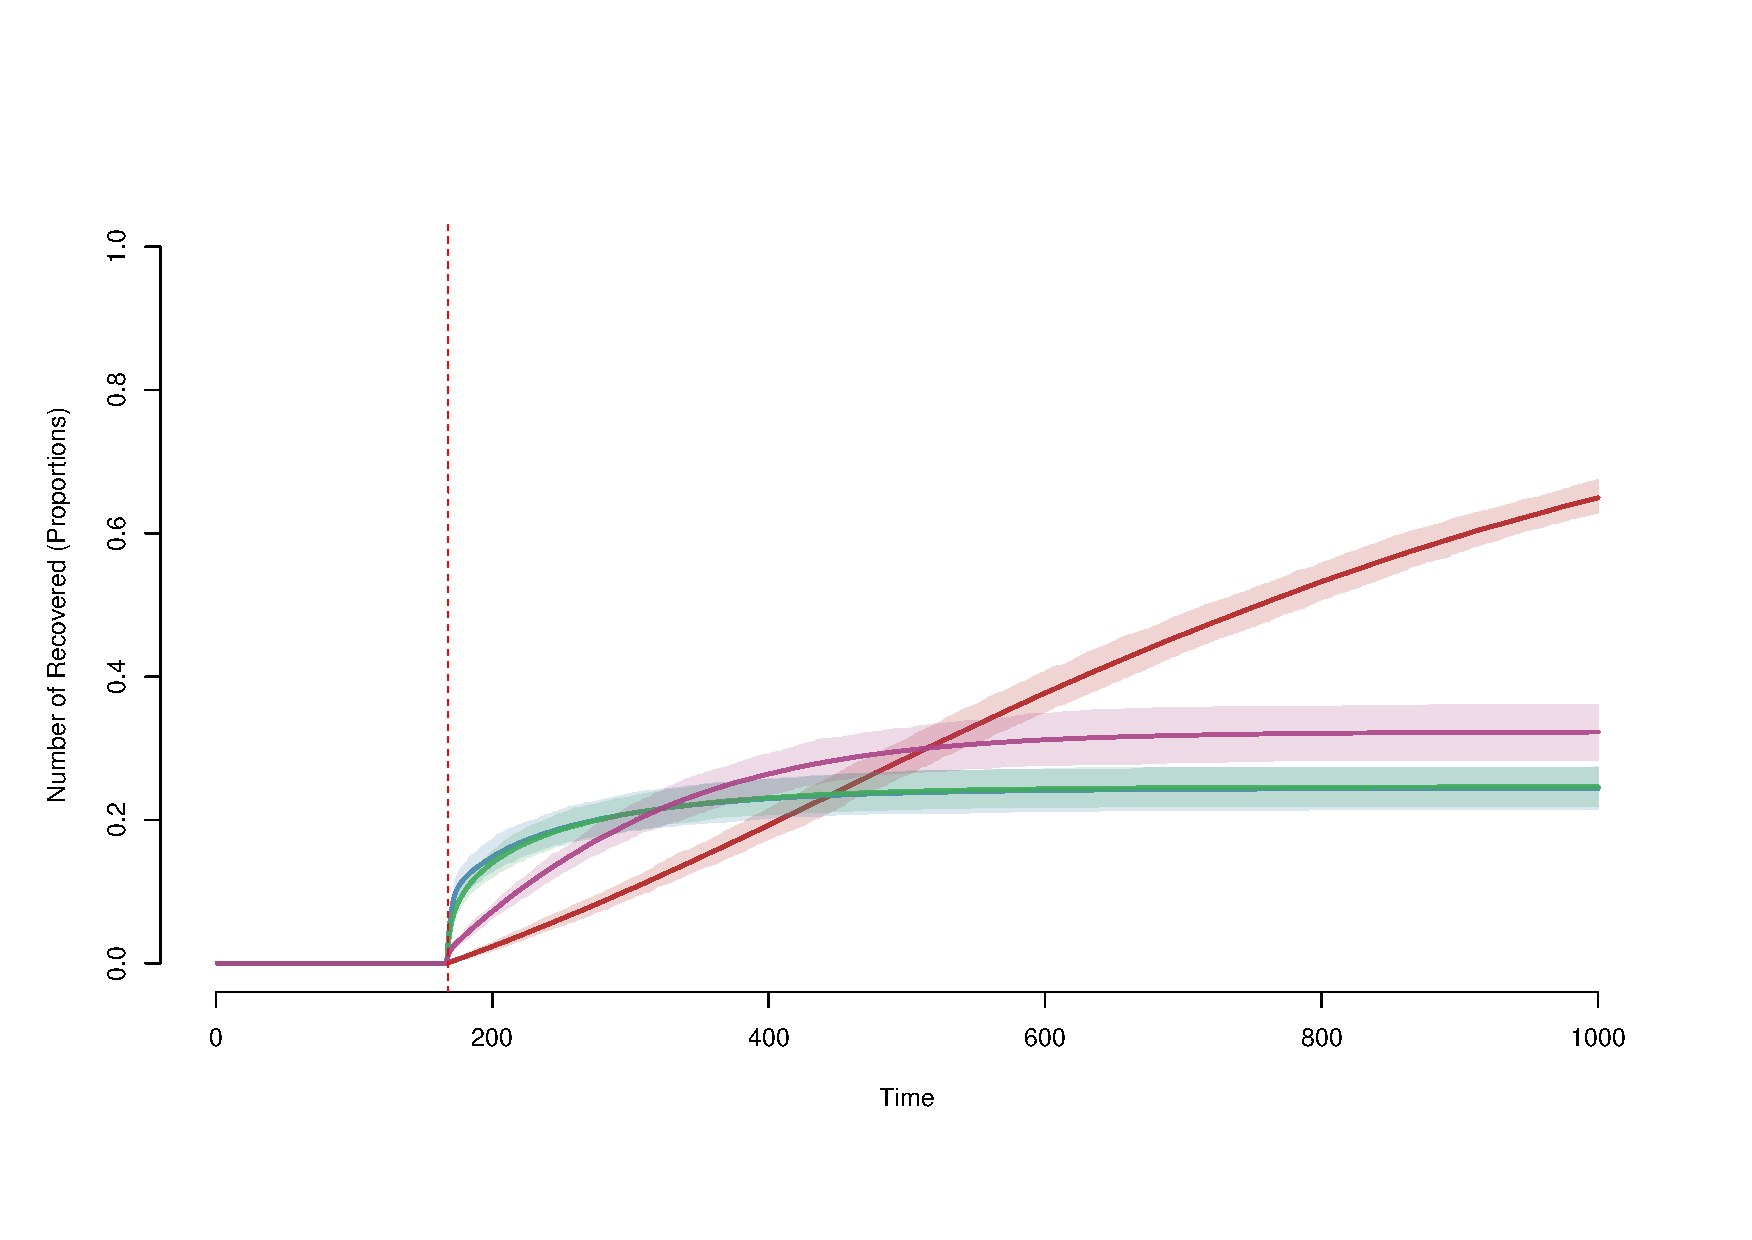
\includegraphics[trim={1.5cm 2.7cm 2cm 5cm}, clip, width=\linewidth]{draft/Fig3d.pdf} 
        \caption*{D. Baseline small-world network} \label{fig3:smallworld}
    \end{subfigure}
    
    \vspace{1cm}
    \captionsetup{format=hang}
    \caption{Proportion of Being Recovered from Infection Status, by Network Topologies} 
    \label{fig:Figure3}
    \captionsetup{font=small}
    \caption*{Note: Red: Asocial random correction, Blue: Thresholds = 0.25, Green: Thresholds = 0.50, and Violet: Thresholds = 0.75.} 
\end{sidewaysfigure}
    
  As can be seen in Figure \ref{fig:Figure3}, all of the social-based correction models produced more effective results in deterring misinformation propagation in the onset of correction intervention. As time progresses, however, across all of the network topologies we instead see asocial random correction models tend to produce more number of being recovered from misinformation infection. However, this is due to the fact that in such scenarios, the number of those who are being \emph{infected} are also larger than threshold-based correction scenarios -- since the number of being recovered is dependent upon the number of being infected at previous time point, even seemingly effective correction settings may produce much fewer cases of being recovered if it had averted new infection at the first place. Therefore, instead of looking at cumulative mean \emph{prevalences} over time, Figure \ref{fig:Figure4} below alternatively present Proportions of infections being averted (PIA) relative to no-recovery scenarios reported in Table \ref{tab:Table3}. For this metric, we derive the proportion of those who otherwise being infected if no recovery had been taken place at each simulated time point as follow: 
\[ PIA_{t} = \frac{I_{t}^{baseline} - I_{t}^{recover}}{I_{t}^{baseline}} \] where $\mathit{I}$ is the number of those who are infected in each of the recovery scenarios $I^{recover}$ (as in Table \ref{tab:Table2}) vs. no-recovery scenarios $I^{baseline}$ (as in Table \ref{tab:Table3}) at each simulated hours $\mathit{t}$. Since no-recovery scenarios reported in Table \ref{tab:Table3} are based on the same network typologies and model specifications \emph{except} infection recovery settings, this allow us to empirically identify counterfactuals without hypothetically assuming number of those who stay being infected. We first derive PIA values for each simulated time points (from time 1 to time 1000), and then take the mean across all time points, then replicate this estimate across 100 simulations per model, as plotted in Figure \ref{fig:Figure4}.  

  As can be seen in Figure \ref{fig:Figure4}, our results reveal that in all of the network topologies, socially-contingent corrections  produce much more effective intervention results than compared to asocial corrections typically considered in extant literature. All of the asocial correction scenarios yield on average PIA values of .46 to .47, whereas all thresholds-based models typically yield PIA values of .74 to .80, meaning on average across all time points, 74 to 80\% of those who otherwise being stay infected and/or newly infected can be prevented based on social-based correction messages exposure and complex contagion of such messages. This appears to be the function of the fact that, in earlier onset of correction message exposure, thresholds values required to adopt correction messages are likely to be easily met due to the scarcity of misinformation in one's immediate environments, therefore attitudinal compositions surrounding simple contagion of misinformation vs. complex contagion of corrective messages tends to favor complex contagion dynamics. This is also evident in Figure \ref{fig:Figure4}, where models with much higher threshold value (=.75, in recovery model 4, model 8, model 12 and model 16) are slightly less effective than other threshold-based models. However, it is indeed interesting to observe that even relatively low threshold (=.25) and moderate threshold (=.50) values all social correction models greatly enhance the effectiveness of corrective message exposure and their adoption.  
  
% Figure 4
\begin{sidewaysfigure}
\captionsetup[figure]{labelfont={bf,it}}
    \centering
        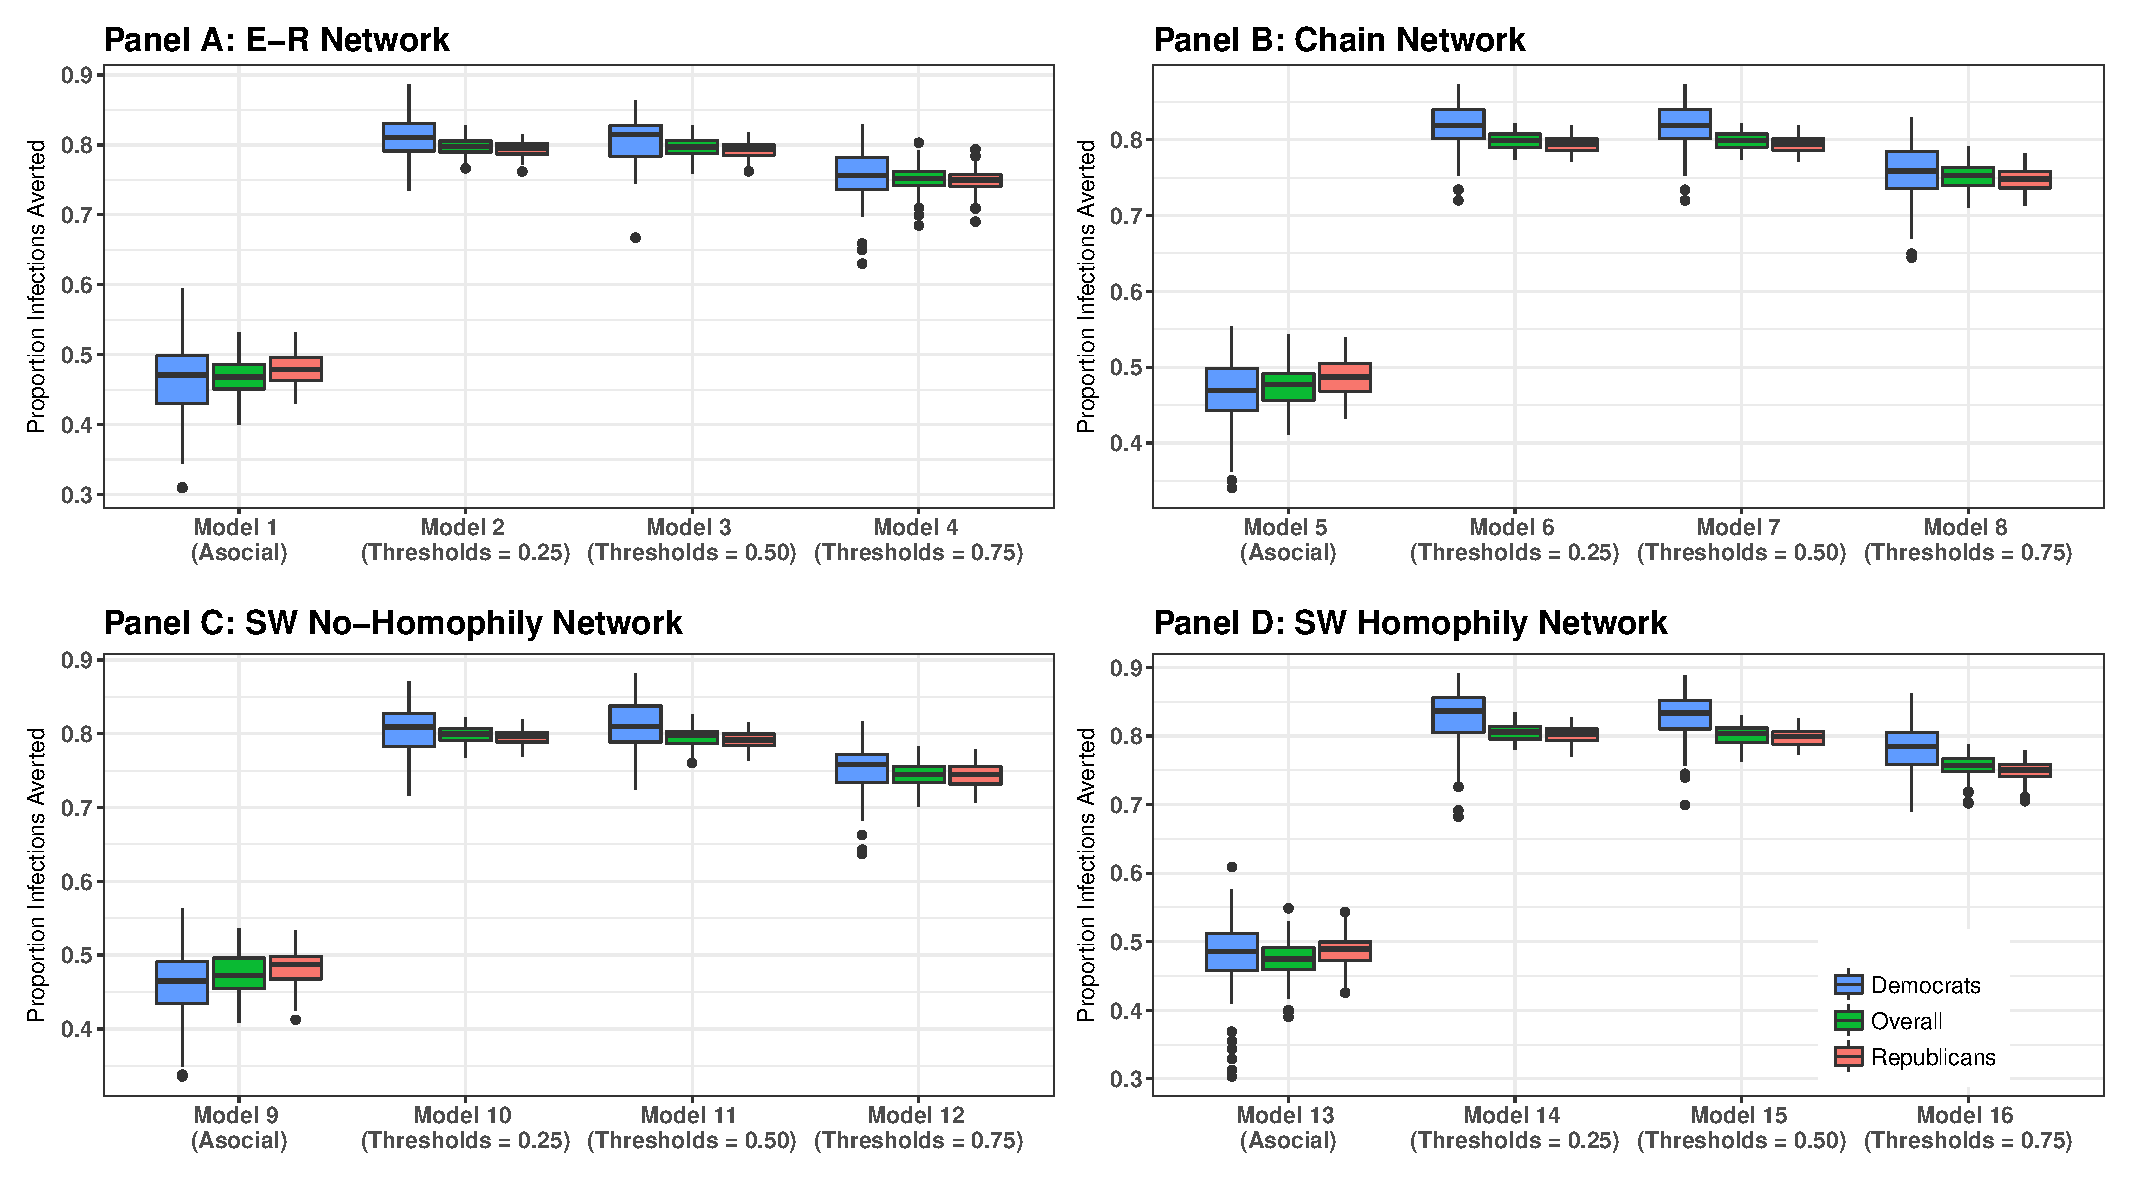
\includegraphics[clip, width=\linewidth]{draft/Fig4.eps} 

    \captionsetup{format=hang}
    \caption{Proportions Infections Averted, Across Recovery Model Thresholds.} 
    \label{fig:Figure4}
    \captionsetup{font=small}
    \caption*{Note: Y-axis denotes Proportions of Infections being Averted (PIA) relative to the no-recovery scenarios. We present overall (= green boxplots), among Democrats (= blue boxplots) and among Republicans (= red boxplots) PIA estimates.} 
\end{sidewaysfigure}        
        
\subsection{Sensitivity Analysis}
  Since we simply assumed the probability of alters sending corrections messages to an infected ego to be .5 in our main results, a series of sensitivity analysis were conducted in order to evaluate the influence of this parameter on the level of PIA metric. In the analyses, probabilities of alters sending corrections to an infected ego were varied to be 0.25 vs. 0.5 vs. 0.75. Figure \ref{fig:Figure5} below reports the results of this sensitivity analysis. Both factors appear to have some impact on PIA estimates, yet at the low to average thresholds models (i.e., models that assume thresholds of adopting corrective messages to be 0.25 or 0.5), the probability of alters sending correction messages did not greatly alter the reported findings in Figure \ref{fig:Figure4}. In the high thresholds models (=0.75, blue plots in Figure \ref{fig:Figure5}), we see the the increased thresholds specification marginally decreases the PIA, yet the higher value of probability of sending corrections appeared to mitigate the effect of higher threshold parameters, especially in our baseline small-world homophily network models (model 14 to model 16 in Table \ref{tab:Table2}). In all of the models, however, PIA metrics are still substantially higher than single-shot, asocial correction scenarios (typically from .46 to .47).     
    
% Figure 5
\begin{sidewaysfigure}
\captionsetup[figure]{labelfont={bf,it}}
    \centering
        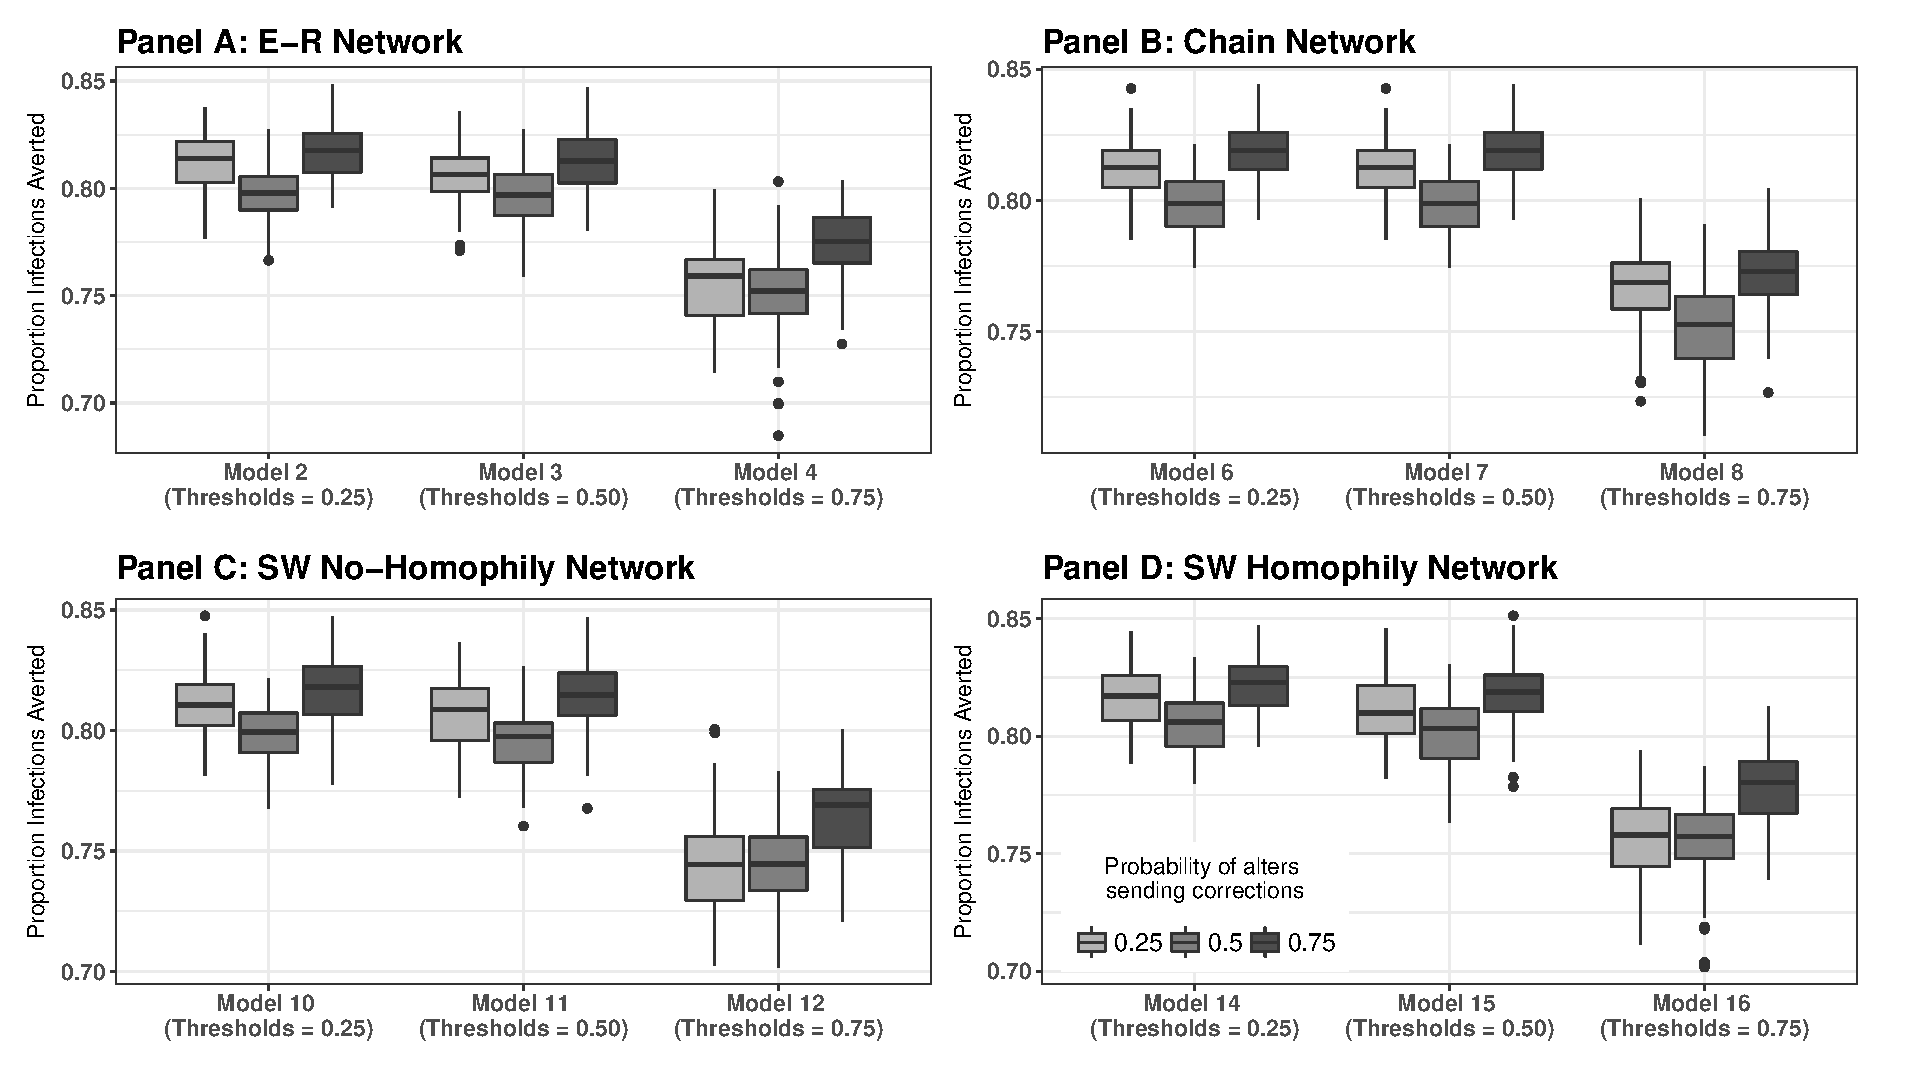
\includegraphics[clip, width=0.9\linewidth, height=0.55\textwidth]{draft/Fig5.eps} 

    \captionsetup{format=hang}
    \caption{Sensitivity Analysis of Alter Probability of Sending Correction Messages, Across Different Recovery Model Thresholds.} 
    \label{fig:Figure5}
    \captionsetup{font=small}
    \caption*{Note: Y-axis denotes Proportions of Infections being Averted (PIA) relative to the no-recovery scenarios. We present different PIA values per each recovery scenario assuming probabilities of alters sending correction messages to infected ego equal to 0.25 (= light gray boxplots), 0.5 (= gray boxplots) and 0.75 (= dark gray boxplots). Main results reported in \ref{fig:Figure4} assumed probability of alter sending corrections to be 0.5 (= gray boxplots).} 
\end{sidewaysfigure}       
  
\section{Discussion and Conclusion}
  Within the context of a misinformation propagation and the adoption of correction messages in social networks, the present study attempted to examine system-level consequences of simple vs. complex contagion dynamics, focusing on the differences between a simple contagion of misinformation and a complex contagion of fact-checking and corrective messages. We further explore boundary conditions that may affect such complex contagion dynamics, focusing different threshold values of adopting corrective messages and its consequences of misinformation propagation at system level outcomes. Utilizing ABM simulations with stochastic network evolution models, this study further highlights the utility of computational social science approaches in robustly exploring various theoretical conditions that otherwise empirically intractable, overcoming the limitations of typical experimental and observations studies concerning complex social phenomena.
    
\subsection{Limitations}
  Before discussing possible implications of our findings, few limitations should be acknowledged. First, due to limitations of available data, our results are bounded by few pure hypothetical (yet still plausible) parameter specifications assumed in simulations, although where available, we have augmented our several key parameter specifications with best-available empirical evidence to date. While more thorough empirical investigation on this topic may further illuminate many aspects of misinformation propagation, our thought-experiment using agent-based simulation further clarifies potential blind spots that need of further research on this topic. Relatedly, our current specifications of simple vs. complex contagion dynamics do not consider how individuals actually process such messages (as would be in controlled experiments) due to much abstract nature of mathematical simulations. 
    
    Second, it should be acknowledged that during our simulations, we treated individuals social network ``links'' as a relatively stable conduit in which specific misinformations and corrections are communicated. Due to such conceptualization, we did not consider the possibility that individuals may end up terminate ties due to misinformation and correction itself -- what we would call ``unfriending'' \parencite{yang2017politics, noel2011unfriending} -- but only considered the possibility of tie dissolution based on more general partisanship (e.g., ties between democrats and republicans are less durable than ties between copartisans). Although such politically motivated, misinformation-based unfriending is somewhat likely, we do not know much about such phenomena in question, let alone its prevalence and mechanisms that enable us to consider such factors in our simulation specifications.
    
    Lastly, the generalizability of these models is partially subject to the underlying behavioral data sources (i.e., 2009 ANES) upon which the baseline models were calibrated. In particular, the level of partisan homogeneity, one of the key theoretical factor of which influence population-level propagation dynamics both in a simple contagion of misinformation and a complex contagion of correction messages, might have been pan out differently had we been able to use a large-scale online social network data that is specifically designed to assess the impact of contagion dynamics concerning misinformation and its correction. While recent contributions on this topic increasingly attempt to directly utilize a large-scale online network data in this regard \parencite[e.g.,][]{Bakshy_2012, del2016spreading}, they typically do not observe propagation of misinformation directly. Such data, typically from Twitter retweet relations or from Facebook Graph API, only provide information between visibly connected dyads (i.e., post-reply relations between actors i and j). Thus, exposure to a message is observed only when actor i ``replies'' or ``follows'' \emph{after} reading actor j’s message. In contrast, unobtrusively tracked behavioral data regarding one's ``exposure'' to specific misinformation (or its correction) is often not available to researchers due to proprietary nature of such data, let alone obtaining such data involves many ethical concerns for researchers \parencite[e.g.,][]{Kramer8788}.  
    
\subsection{Implications}
     Overall, our simulation results confirm our initial expectation that socially-contingent corrections are substantially more, if not equally, effective in preventing a given misinformation to further propagate into public. Following discussions of complex and ``contested'' contagion dynamics \parencite{centola2007complex, Centola2010Sience, Centola2007449, gonzalez2017decoding}, we argued that individuals are more likely to accept socially-provided correction messages \parencite[e.g.,][]{margolin2017, bode2017see}, and as a consequence, social correction scenarios would be more effective than a single-shot, asocial correction that typically have been considered in extant literature. Although in a realistically defined, baseline network misinformation appear to be spread more faster than pure random networks or than non-homophilic network (Figure \ref{fig:Figure2}), once corrections are introduced into the network, the baseline topology was indeed capable of deterring the spread of misinformation more effectively (measured by proportions of infections being averted) than any other counterfactual network topologies (Figure \ref{fig:Figure4}). This appears due to the fact that socially-contingent correction dynamics are more effective in preventing a small number of existing misinformation infection at the earlier stage of the misinformation propagation.    

    Our results also reveal that currently specified social correction models are relatively robust against potential variations in specific threshold values of adopting complex (contested) contagions (0.25 vs. 0.5 vs. 0.75) and probabilities of one's alters actually sending corrections to infected individuals (again, 0.25 vs. 0.5 vs. 0.75: see our results in ``Sensitivity Analysis'', Figure \ref{fig:Figure5}). We observed that largely equivalent proportions of infections being averted due to corrections even in models with relatively high-adoption thresholds coupled with low probability of alters sending actual corrections to an infected ego. This may further be seen as implying that the social cost of sending corrective messages to one's peers play a rather limited role in complex contagion dynamics at least in the current framework. Yet considering the fact that friend-friend corrections may entail certain relational costs when in comes to sending (misinformation) correction messages -- such as topic avoidance \parencite{morey2012matters} or even political unfriending \parencite{yang2017politics, noel2011unfriending}, these findings does not necessarily imply the unimportance of social costs of sending corrections and how frequent such corrections are received by misinformed individuals. Quite contrary, our results imply \emph{as long as individuals keep maintain} some degree of attitudinally diverse social connections, the effectiveness of socially-contingent corrections would remain robust to such factors. 
    
    Now there are good reasons to believe that individuals do not selectively construct their political environments simply based on their partisan similarity \parencite{morey2012matters, lazer2010coevolution, song2015uncovering}. Even in online settings one may be exposed to nontrivial degree of counter-attitudinal information \parencite[e.g.,][]{Bakshy_2012, messing2014selective}. Under such conditions, the social network relations -- as opposed to asocial corrections from strangers -- may stimulate more effective individual- and population-level outcomes of fact-checking messages \parencite[e.g.,][]{margolin2017, bode2017see}. Yet at the same time, these findings might be unexpected if individuals indeed form their social relations purposively through their political and ideological similarities, therefore limiting the possibility of receiving independent, multiple reinforcements of corrective messages targeting misinformation. While a real-world replication with much more detailed data, beyond this particular simulation context, would provide firm evidence on the generalizability of our findings, it is our hope that the current investigation would illuminate further scholarly effort of investigating when and how corrections to misinformations can contribute to the ideals of informed citizenly.

\printbibliography
\newpage
\begingroup
\parindent 0pt
\parskip 1ex
\def\enotesize{\normalsize}
\theendnotes
\endgroup
\end{document}
